\documentclass[10pt,journal,compsoc]{IEEEtran}
% Load basic packages
\usepackage{balance}  % to better equalize the last page
\usepackage{graphics} % for EPS, load graphicx instead
\usepackage[T1]{fontenc}
% \usepackage{txfonts}
% \usepackage{mathptmx}
\usepackage[pdftex]{hyperref}
\usepackage{color}
\usepackage{xcolor}
\usepackage{booktabs}
\usepackage{textcomp}
\usepackage{xspace}
\usepackage{setspace}
\usepackage[textsize=tiny]{todonotes}
% Some optional stuff you might like/need.
\usepackage{microtype} % Improved Tracking and Kerning
% \usepackage[all]{hypcap}  % Fixes bug in hyperref caption linking
\usepackage{ccicons}  % Cite your images correctly!
% \usepackage[utf8]{inputenc} % for a UTF8 editor only
\usepackage{verbatim}
\usepackage{relsize}
\usepackage{etoolbox}
\usepackage{lipsum}   % for filler text
\usepackage{setspace} % for \onehalfspacing and \singlespacing macros
\usepackage[normalem]{ulem}
\usepackage[sort,nocompress]{cite}
\usepackage{xcolor}
\usepackage{fixltx2e}
\usepackage{amsmath}
\usepackage{amssymb}
\usepackage{afterpage}
\usepackage{microtype}                 % use micro-typography (slightly more compact, better to read)
\PassOptionsToPackage{warn}{textcomp}  % to address font issues with \textrightarrow
\usepackage{times}                     % we use Times as the main font
\renewcommand*\ttdefault{txtt}         % a nicer typewriter font
\usepackage{cite}                      % needed to automatically sort the references
\usepackage{tabu}                      % only used for the table example
\usepackage{booktabs}                  % only used for the table example
% \usepackage[linesnumbered,ruled]{algorithm2e}
\usepackage{algorithm}
\usepackage[noend]{algpseudocode}

\usepackage{tikz}
\usetikzlibrary{shapes,arrows}
\usepackage{subfig}
\captionsetup{belowskip=-5pt,aboveskip=5pt}
% \BeforeBeginEnvironment{table}{\vskip-1ex}
% \AfterEndEnvironment{table}{\vskip-1ex}

\DeclareMathOperator*{\argmax}{arg\,max}
% llt: Define a global style for URLs, rather that the default one
\makeatletter
\def\url@leostyle{%
  \@ifundefined{selectfont}{
    \def\UrlFont{\sf}
  }{
    \def\UrlFont{\small\bf\ttfamily}
  }}
\makeatother

\newenvironment{denselist}{
    \begin{list}{\small{$\bullet$}}%
    {\setlength{\itemsep}{0ex} \setlength{\topsep}{0ex}
    \setlength{\parsep}{0pt} \setlength{\itemindent}{0pt}
    \setlength{\leftmargin}{1.5em}
    \setlength{\partopsep}{0pt}}}%
    {\end{list}}

\newcommand{\squishlist}{
   \begin{list}{$\bullet$}
    { \setlength{\itemsep}{0pt}
      \setlength{\parsep}{2pt}
      \setlength{\topsep}{0pt}
      \setlength{\partopsep}{0pt}
      \leftmargin=25pt
\rightmargin=0pt
\labelsep=5pt
\labelwidth=10pt
\itemindent=0pt
\listparindent=0pt
\itemsep=\parsep
    }
}
\newcommand{\squishend}{\end{list}}
\newcommand{\npar}{\par \noindent}
% use extensively to toggle between paper and TR
\newcommand{\eat}[1]{}
% \newcommand{\papertext}[1]{{\leavevmode\color{blue}{#1}}}
% \newcommand{\techreport}[1]{{\leavevmode\color{red}{#1}}}
\newcommand{\papertext}[1]{#1}
\newcommand{\techreport}[1]{}
\newcommand{\boldpara}[1]{\textbf{\paragraph{#1}}}
% de-facto paragraph format
\newcommand{\stitle}[1]{\par\noindent\textbf{#1}}
\newcommand{\tvcg}[1]{{\leavevmode\color{blue}{#1}}}
\newcommand{\cut}[1]{{\leavevmode\color{lightgray}{#1}}}
\newcommand{\ccut}[1]{} %confirmed cut
\newcommand{\system}{\textsc{Storyboard}\xspace}
\newcommand{\cluster}{\textsc{Cluster}\xspace}
\newcommand{\BFS}{\textsc{BFS}\xspace}
\def\plaintitle{\system : Hierarchical Summary of Equivalent Visualizations across Data Subsets}
\def\plainauthor{Doris Jung-Lin Lee*, Himel Dev*, Huizi Hu, Hazem Elmeleegy, Aditya Parameswaran}
\def\emptyauthor{}
\def\plainkeywords{Data visualization, exploratory data analysis, visual query, scientific data.}
\def\plaingeneralterms{Documentation, Standardization}

\newcommand{\agp}[1]{\textcolor{blue}{Aditya: #1}}
\newcommand{\dor}[1]{\textcolor{green}{Doris: #1}}
\newcommand{\hdev}[1]{\textcolor{magenta}{Himel: #1}}
\newcommand{\haz}[1]{\textcolor{orange}{Hazem: #1}}
\newcommand\notes[1]{\textcolor{red}{#1}}
\urlstyle{leo}
\AtBeginEnvironment{quote}{\small}
% To make various LaTeX processors do the right thing with page size.
\def\pprw{8.5in}
\def\pprh{11in}
\special{papersize=\pprw,\pprh}
\setlength{\paperwidth}{\pprw}
\setlength{\paperheight}{\pprh}
\setlength{\pdfpagewidth}{\pprw}
\setlength{\pdfpageheight}{\pprh}

% Make sure hyperref comes last of your loaded packages, to give it a
% fighting chance of not being over-written, since its job is to
% redefine many LaTeX commands.
\definecolor{linkColor}{RGB}{6,125,233}
\hypersetup{%
  pdftitle={\plaintitle},
% Use \plainauthor for final version.
%  pdfauthor={\plainauthor},
  pdfauthor={\emptyauthor},
  pdfkeywords={\plainkeywords},
  bookmarksnumbered,
  pdfstartview={FitH},
  colorlinks,
  citecolor=black,
  filecolor=black,
  linkcolor=black,
  urlcolor=linkColor,
  breaklinks=true}


% Get rid of gaps between sections, subsections and subsubsections
% \usepackage{titlesec}
% \titlespacing*{\section}
% {0pt}{0pt}{0pt}
% \titlespacing*{\subsection}
% {0pt}{0pt}{0pt}
% \titlespacing*{\subsubsection}
% {0pt}{0pt}{0pt}
% End of preamble. Here it comes the document.

\ifpdf%                                % if we use pdflatex
  \pdfoutput=1\relax                   % create PDFs from pdfLaTeX
  \pdfcompresslevel=9                  % PDF Compression
  \pdfoptionpdfminorversion=7          % create PDF 1.7
  \ExecuteOptions{pdftex}
  \usepackage{graphicx}                % allow us to embed graphics files
  \DeclareGraphicsExtensions{.pdf,.png,.jpg,.jpeg} % for pdflatex we expect .pdf, .png, or .jpg files
\else%                                 % else we use pure latex
  \ExecuteOptions{dvips}
  \usepackage{graphicx}                % allow us to embed graphics files
  \DeclareGraphicsExtensions{.eps}     % for  pure latex we expect eps files
\fi%

%% it is recomended to use ``\autoref{sec:bla}'' instead of ``Figure ~\ref{sec:bla}''
\graphicspath{{figures/}{pictures/}{images/}{./}} % where to search for the images

%%%%%%%%%%%%%%%%%%%%%%%%%%%%%%%%%%%%%%%%%%%%%%%%%%%%%%%%%%%%%%%%
%%%%%%%%%%%%%%%%%%%%%% START OF THE PAPER %%%%%%%%%%%%%%%%%%%%%%
%%%%%%%%%%%%%%%%%%%%%%%%%%%%%%%%%%%%%%%%%%%%%%%%%%%%%%%%%%%%%%%%%

\begin{document}
\title{\system : Navigating Through Data Slices with Hierarchical Summary of Visualizations}
\author{\plainauthor}
% \IEEEcompsocitemizethanks{ \IEEEcompsocthanksitem The authors are with University of Illinois, Urbana-Champaign. Hazem Elmeleegy is with Amobee Inc.
%  \protect\\ E-mail: jlee782, hdev3, huizihu2, skuzi2, adityagp@illinois.edu. hazem.elmeleegy@amobee.com.
% }
\IEEEtitleabstractindextext{%
\begin{abstract}
The task of navigating through a large, multidimensional dataset is a common challenge in exploratory analysis. Not only is manual drill-down and roll-up on data subsets tedious and inefficient for the analyst, the massive space of data subsets, lack of interesting patterns in most data subsets, fallacies of spurious correlations, and pitfalls of statistical paradoxes calls for a systematic and effective way for an analyst to make sense of and navigate through the large space of possible visualizations. In this paper, we present \system, an interactive visualization recommendation system that automatically identifies k connected visualizations that summarizes the interesting and informative trends in the dataset to the user. Given a dataset and the x and y axes of interest, \system\ intelligently explores the lattice of equivalent visualizations across data subsets, and recommends interesting and informative visualizations based on an intuitive user-expectation model. The recommended visualizations are then displayed in an interactive dashboard, where the visualizations are organized into a hierarchical layout. Our evaluation study shows that visualization dashboards generated by \system\ are interpretable and leads to higher performance in data analytic tasks compared to the competing baselines.
%%\abstract{The task of navigating through a large, multidimensional dataset is a common challenge in data analytics. Not only is manual drill-down and roll-up on data subsets tedious and inefficient for the analyst, but even with all the information given, there is no systematic and effective way for an analyst to make sense of and navigate through the large space of possible visualizations. We present \system, an interactive visualization recommendation system that automatically selects k visualizations to tell an interesting, connected, and informative story to the user. Given a dataset, \system\ intelligently explores a lattice of equivalent visualizations across data subsets and recommend visualizations based on an intuitive user-expectation model. The recommended visualization is displayed in an interactive dashboard where the visualizations are organized into hierarchical graph layout. Our evaluation study shows that visualization dashboards generated by \system\ were more interpretable and resulted in higher performance in data analytic tasks among our users compared to other competing baselines.}
%- interactivity claim? 
%\title{Navigating Filter Space with \system : Informative and Insightful Summary of Visualizations across Data Subsets}
%\abstract{Searching for similar (and dissimilar) patterns in hundreds of data subsets is a common exercise in many data science tasks, including feature selection, outlier detection, and funnel analysis. There are several challenges that makes this exercise particularly hard---the massive space of data subsets (even for a modest dataset with a few hundred attributes), the lack of interesting patterns in most data subsets, the fallacies of spurious correlations, the pitfalls of statistical paradoxes (e.g., Simpson's paradox) are some of the key challenges. In this paper, we present \system , an interactive visualization recommendation system that automates the \lq\lq pattern exploration\rq\rq\ exercise by presenting an interesting and informative summary of trends to the user. Given a dataset and the x and y axes of interest, \system\ intelligently explores the lattice of equivalent visualizations across data subsets, and recommends interesting and informative visualizations based on an intuitive user-expectation model. The recommended visualizations are then displayed in an interactive dashboard, where the visualizations are organized into a hierarchical layout. We performed an extensive user study to show that the dashboards generated by \system\ are interpretable and leads to higher performance in data analytic tasks compared to the competing baselines.}
%\title{\system : Interactive Exploration of Data Slices Through Hierarchical Summary Visualizations}
%Not only is manual drill-down and roll-up on data subsets tedious and inefficient for the analyst, but even with all the information given, there is no systematic and effective way for an analyst to make sense of and navigate through the large space of possible visualizations. We present \system, an interactive visualization recommendation system that automatically selects k visualizations to tell an interesting, connected, and informative story to the user. Given a dataset, \system\ intelligently explores a lattice of equivalent visualizations across data subsets and recommend visualizations based on an intuitive user-expectation model. The recommended visualization is displayed in an interactive dashboard where the visualizations are organized into hierarchical graph layout. Our evaluation study shows that visualization dashboards generated by \system\ were more interpretable and resulted in higher performance in data analytic tasks among our users compared to other competing baselines.}
\end{abstract}

\begin{IEEEkeywords}
exploratory data analysis, visualization recommendation.
\end{IEEEkeywords}}

% make the title area
\maketitle


% To allow for easy dual compilation without having to reenter the
% abstract/keywords data, the \IEEEtitleabstractindextext text will
% not be used in maketitle, but will appear (i.e., to be "transported")
% here as \IEEEdisplaynontitleabstractindextext when the compsoc
% or transmag modes are not selected <OR> if conference mode is selected
% - because all conference papers position the abstract like regular
% papers do.
\IEEEdisplaynontitleabstractindextext
% \IEEEdisplaynontitleabstractindextext has no effect when using
% compsoc or transmag under a non-conference mode.


\begin{figure*}[bht]
\centering
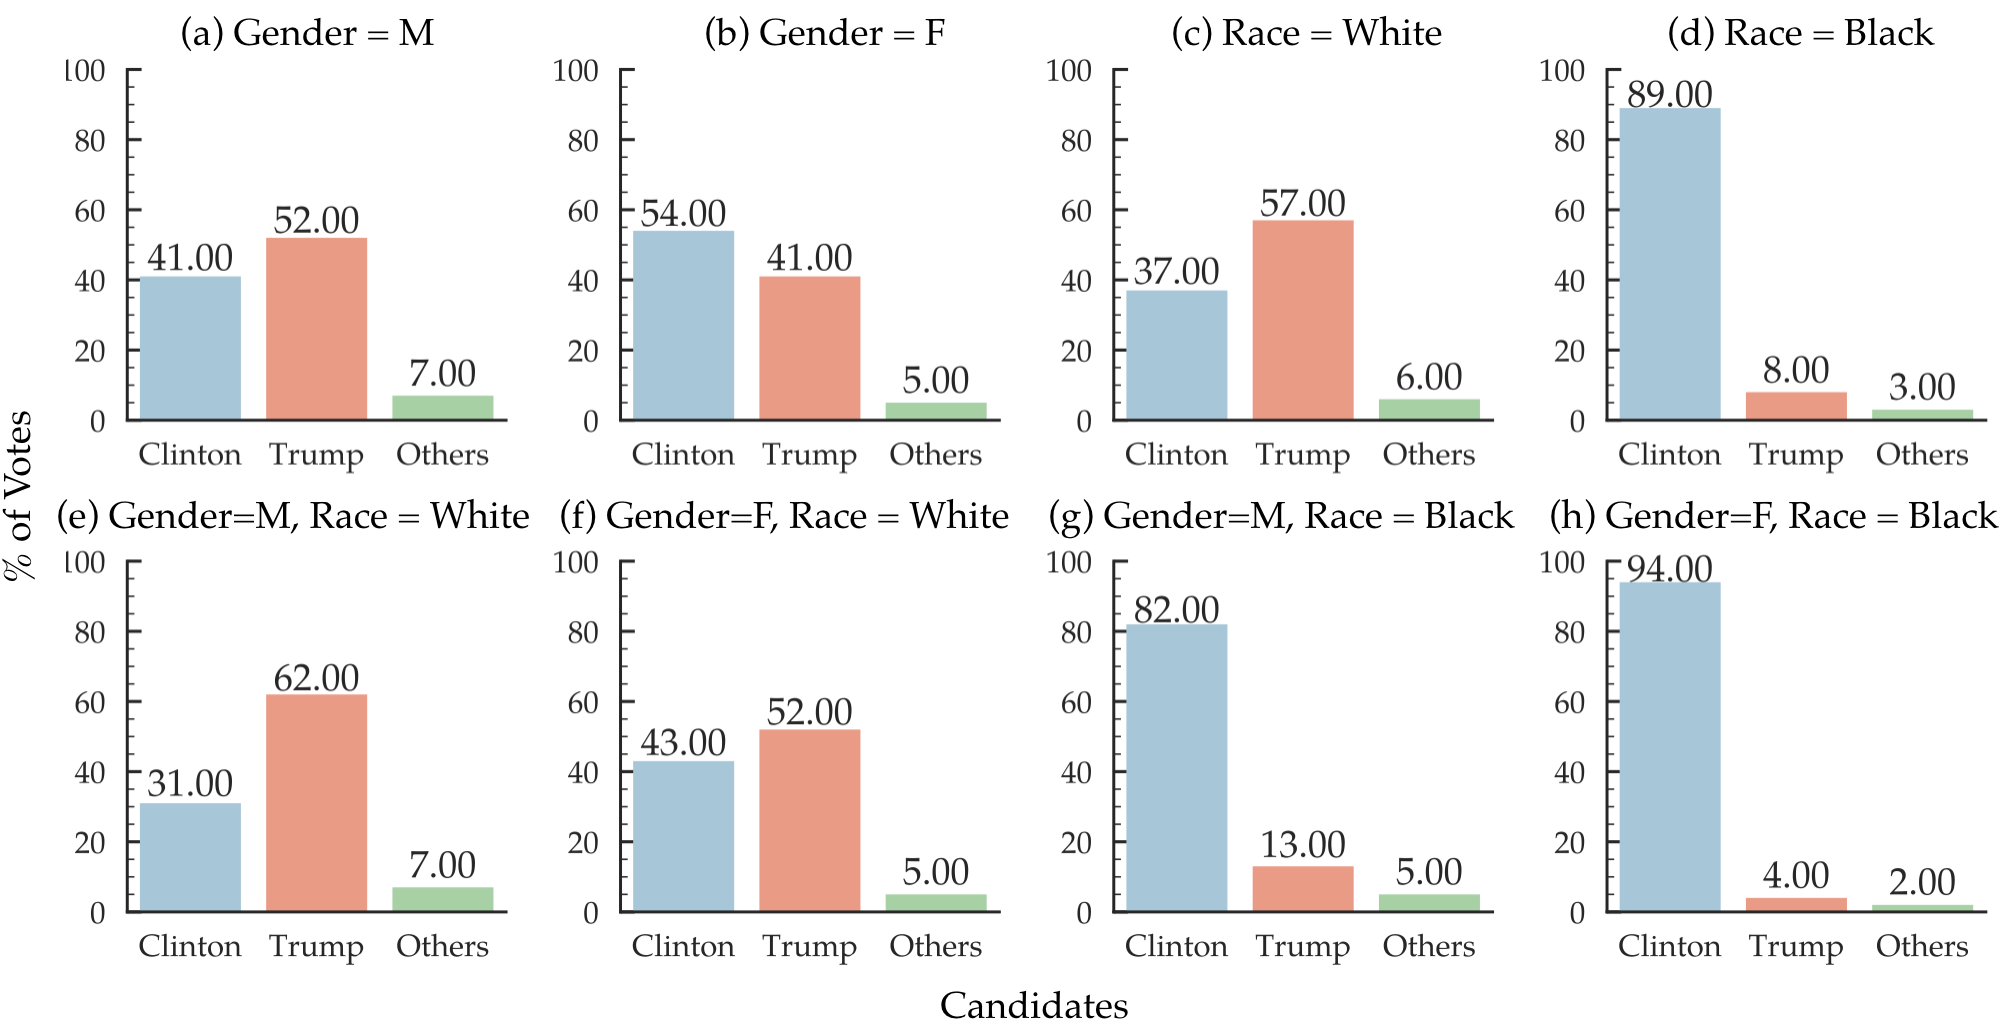
\includegraphics[width=\linewidth]{figures/US_Election_Example.png}
\caption{A set of visualizations from the 2016 Election polls. These visualizations show the percentage of votes for three candidates (Donald Trump, Hilary Clinton, and Others) in different demographic groups (based on race and gender).}
\label{fig:elections_example}
\end{figure*}

\section{Introduction}

%\hdev{Let's take a step back, and look at the current flow in introduction. In the first paragraph, we vaguely motivate what can be considered as collective insights. In second paragraph, we try to connect the idea of collective insights with the challenges of data subset exploration. In third paragraph, we introduce two concepts: visual summarization, and distribution awareness. We do not clearly state what these two means. There's an example that conveys what could be captured through pattern or trend mining. In the fourth paragraph, we present an example to convey some specific challenges of visual summarization. The fifth paragraph states our contributions. My suggestion is to immediately jump into business by saying what we mean by distribution awareness, why is it important, and why is this challenging. We have the contents lying around already, it's just a matter of clearly stating these three aspects, preferably without using new abstractions.}

Common analytics tasks, such as causal inference, feature selection, and outlier detection requires studying the distributions or patterns at different granularities of data [Refs]. For example, a campaign manager may study the voting patterns in different demographics (based on race, gender, social class etc.) using the 2016 US election exit polls\footnote{\url{https://edition.cnn.com/election/2016/results/exit-polls}} to identify the nonconformist demographic groups. Visual analysis is the \emph{de facto} approach for performing such analytics tasks [Refs], where an analyst constructs visualizations to capture the distributions at different subsets of data. The goal of this visual analysis is to extract meaningful insights---when a set of visualizations along with human interpretation leads to informative and interesting facts arising from the distributions.

However, without knowing \textit{what} subset of data contains an interesting distribution, manually exploring all possible data subsets can be tedious and inefficient for an analyst. For example, the aforementioned campaign manager could construct bar charts for different demographics, where x-axis shows the election candidates and y-axis the percentage of votes for these candidates. Subsequently, he could compare these bar charts to understand how voting pattern changes across different demographics. Both of these exercises, first, constructing the large number of visualizations corresponding to all possible data subsets, and then, navigating through this large space of visualizations to draw meaningful insights is challenging. Currently, there is no systematic way to perform these exercises. 

To this end, we present \system, an interactive visualization summarization system that automatically selects a small set of visualizations to summarize the data distributions within a dataset in an informative manner. When analysts inspect informative visualizations that cover these insights, they associate particular sets of attributes to typical trends and observed patterns. We define this aspect of dataset understanding as \emph{distribution awareness}. For example, we observe that in Figure~\ref{fig:elections_example}, most of the visualizations has `Clinton' and `Trump' as comparably-sized bars with `Others' being a small fraction of the overall (a,b,c,e,f), whereas visualizations involving the Black population is highly skewed towards `Clinton' (d,g,h). Since human analysts have limited memory and attention, it is often impossible to visualize all possible data subsets. An ideal summarization system should display visualizations that enables users to gain maximal distribution awareness of the typical trends within a dataset. 

%Even after constructing the visualizations for all possible data subsets, which itself is a daunting task, currently there is no systematic way for our campaign manager to make sense of or even navigate through this large space of possible visualizations to draw meaningful insights. 

%\par The goal of visual analysis is to extract meaningful stories or insights from the data. Individual visualizations represent simple ``factoids'' portraying one aspect of the data. Meaningful insights arise when a group of factoids work in conjunction, along with human interpretation, to produce informative and interesting facts. 
%\par However, without knowing \textit{what} subset of the data would be interesting to visualize, manual drill-downs and roll-ups on all possible filter combinations can be tedious and inefficient for analysts. In many data analytics scenarios, analysts have an x and y axis of interest and want to explore data subsets corresponding to different filtering criteria. For example, a campaign manager may be interested in looking at bar chart visualizations of x as the voted candidate and y as the percentage of votes for the 2016 US elections exit polls with different filter combinations on demographics information, such as gender, income, race, states, and responses to different survey questions\footnote{\url{https://edition.cnn.com/election/2016/results/exit-polls}}. The analyst would have to compare across a combinatorially large space of different data subsets by iteratively changing the filter criterion of a visualization to understand how the relationship between the x and y variables change across data subsets. Even if the analyst had plotted visualizations for all possible data subsets, currently there is no systematic and effective way for an analyst to make sense of and navigate through the large space of possible visualizations to draw meaningful insights. 
%\par To this end, we present \system, an interactive visualization summarization system that automatically selects a small set of visualizations to summarize the data distributions within a dataset in an informative manner. When analysts inspect informative visualizations that cover these insights, they associate particular sets of attributes to typical trends and observed patterns. We define this aspect of dataset understanding as \emph{distribution awareness}. For example, we observe that in Figure~\ref{fig:elections_example}, most of the visualizations has `Clinton' and `Trump' as comparably-sized bars with `Others' being a small fraction of the overall (a,b,c,e,f), whereas visualizations involving the Black population is highly skewed towards `Clinton' (d,g,h). Since human analysts have limited memory and attention, it is often impossible to visualize all possible data subsets. An ideal summarization system should display visualizations that enables users to gain maximal distribution awareness of the typical trends within a dataset. 
%\par However, finding effective visualizations to summarize a dataset is not as trivial as picking individual visualizations that maximizes some statistical measure, such as deviation~\cite{Vartak2015}, coverage~\cite{Sarvghad2017}, or significance testing~\cite{Anand2015}, which can often result in misleading summarizations. Consider an elections campaign manager who is allocating the advertisement budget to be spent on different demographic populations to target for an upcoming election by investigating the voting patterns across different demographic groups. He performs a randomized permutation testing between the gender and race attributes and finds that the voting pattern of black females is drastically different from the voting pattern of general female population and allocates the his advertisement funds to target the black female population. \dor{Himel, can you check if this example makes sense? or should we say chi2? chi2 just give you columnar correlation info not at the attribute-level info? although probably only a deviation based comparison can give you a comparison like this.} While black females do defy the trends of general females, the comparison is incomplete, since it ignores the fact that black females follows very closely to the distribution of the voting behavior of the black population, so the proper subpopulation to target should be the black population rather than the more specific black female population.
%\par The above example showcases a scenario where the selection of an improper reference (female) for comparing the visualization (black female) against results in misleading insights. In \system, we formulate an objective where a visualization is \emph{actually} interesting when it deviates from and can not be explained by \emph{even} its most informative reference. \dor{can we add an example here?} Our user study results described in Section~\ref{sec:userstudy} shows that this notion of informative interestingness can guide an analyst towards more meaningful stories for further investigation. 
\par The contribution of this paper include: 
\begin{denselist}
\item Proposing the novel problem of visualization summarization and use cases highlighting the importance of \textit{distribution awareness} in dataset understanding (Section~\ref{sec:distributionaware}), %inform  visualization understanding and analytical tool designs
\item Formulating the structure and utility of the visualization search space (\emph{lattice}) using a user expectation model motivated by our formative study (Section~\ref{sec:datamodel}),
\item Designing efficient algorithms and optimizations to identify a set of informatively connected interesting visualizations (Section~\ref{sec:system}),  
\item Presenting an interactive visualization dashboard interface that adopts a simple and intuitive hierarchical lattice layout (Section~\ref{sec:interaction}),
\item Demonstrate the efficacy of our system through a user study evaluation (Section~\ref{sec:userstudy}).
\end{denselist}
%!TEX root = main.tex
\section{Distributional awareness and its applications\label{sec:distributionaware}}
The idea of picking a small set of visualizations to summarize the dataset is motivated by the observation that most of the data distributions in a dataset can be explained by a much smaller set of visualization instances\footnote{This principle is more generally known as the 80-20 rule in economics, e.g. 80\% of the wealth (effect) is held by approximately 20\% of the population (cause).}. We define that a set of visualizations instills \emph{ distributional awareness} if the visualization helps analyst understand many of the possible visualization distributions and their associated attribute combinations. The goal of visualization summarization is to assemble a dashboard of $k$ visualizations that help analysts become distributionally aware of other unseen perspectives in the dataset. In addition to accelerating the process of manual comparisons across different data subsets described in the introduction, we illustrate a series of common data analytics tasks that would benefit from enhanced distributional awareness through visualization summarization In this section, we use the popular Titanic dataset as a continued example, commonly used for introducing novices to the classification problem in machine learning\cite{titanic}.
% \npar \textbf{Comparisons across Data Subsets:} In many data analytics scenarios, analysts have an x and y axis of interest and want to explore data subsets corresponding to different filtering criteria. For example, the Titanic dataset contains dimensional attributes (ticket classes, age, and gender) for predicting whether a passenger survives or not survive the shipwreck. The analyst would have to compare across different data subsets by iteratively changing the filter criterion of a visualization to understand how the relationship between the x and y variables change across data subsets.
% \npar Without knowing \textit{what} subset of the data would be interesting to visualize, the manual drill-down and roll-ups on all possible filter combinations can be tedious and inefficient for the analyst. And even if the analyst had plotted visualizations for all possible data subsets, currently there is no systematic and effective way for an analyst to make sense of and navigate through the large space of possible visualizations to draw meaningful insights. \footnote{\cite{anand} is one example of a visualization dashboard demonstrating the insights from exploring through different facets in the Titanic dataset.}
\npar \textbf{Preventing Fallacies in Causal Inference:} Drawing inference from observations is important for discovering causal relationships that support or refute a hypothesis, as well as generalizing predictions for unseen data. During exploratory analysis, causal inference based on the incomplete, aggregate information can result in Simpson's paradox~\cite{Guo2017}, whereby an observed trend between variables reverses when conditioned upon an unseen variable.
\npar One example of Simpson's paradox in the Titanic dataset is the survival rate of passengers for third-class passengers versus crew members. Overall, the survival rate of third-class passengers is slightly higher (24.08\%) than crews (23.95\%). However, when we examine the survival rate of the two classes conditioned on gender as shown in Table.\ref{tab:t2}. We find that for both genders, the survival rate of the crews is higher than third-class passengers.
\begin{table}[thb]
    \label{tab:t2}
	\begin{center}
	\begin{tabular}{ccccc}
	\toprule
	Gender & Class & Survived & Lost & Survival\\
	& & & & Rate\\
	\midrule
	M & Third & 75 & 387 & 16.23\%\\
	M & Crew & 192 & 670 & 22.27\%\\
	\bottomrule
    F & Third & 76 & 89 & 46.06\%\\
	F & Crew & 20 & 3 & 86.96\%\\
	\bottomrule
	\end{tabular}
    \end{center}
	\caption{Survival Rate by Gender and Two Classes}
\end{table}
In this case, Simpson's paradox arises because the gender distribution for each passenger class was not shown, so analysts may be misguided into thinking that survival rates of third-class passengers should be equal or slightly higher than crews. As studied by \cite{Alipourfard2018,Guo2017}, identification of Simpson's paradox is important as it reveals interesting subgroups which differ from their expected behavior--so much that their aggregated trends are reversed. While the goal of \system is not the identification of Simpson's paradox, our goal of helping analysts become distributionally aware of their dataset circumvent this issue, since the displayed visualizations should yield a informative view that covers the main patterns in the data. Furthermore, our objective ensures that for a visualization to be selected in the dashboard at least one of the ``informative parents'' are already in the dashboard to exclude visualizations that could misguide the users into such fallacies.

\npar \textbf{Feature Selection for Machine Learning:} Data scientists often create visualizations to uncover the relationships between their chosen attributes and potential influencer variables to identify attributes that are relevant to the prediction task. Feature selection is a non-trivial problem: analysts seek attribute combinations that are highly discriminative, yet general enough to prevent overfitting and increase model interpretability. While existing classification algorithms such as decision trees highlight some of such cases, as their end-goal is to improve classification score, the reductionist view does not showcase the complex interactions where trends may be changing when additional attributes are added. By becoming distributionally aware of the dataset, analysts can learn key patterns that are associated with particular attributes, such as female passengers on the Titanic has a much higher survival rate than male passengers. As described in the paper, the non-monotonic story paths selected by the context-dependent objective in \system \dor{might be too much to mention this here, consider putting this para after models? or as discussion?} can help users make more informative judgments about feature importance in the given datasets.

\npar \textbf{Contextual Outlier Detection and Interpretation:} In many data-driven applications, outlier detection plays an important role in identifying groups of instances that are different from the majority. Interpreting \textit{why} a particular outlier was chosen is essential for analysts to reason about the underlying phenomenon resulting in the outlier. Female crew member in the Titanic dataset is one example of such outliers, whose high survival rate is different from that of both female (51.06\%) and crews (23.95\%), whereas the female third class passengers can be explained using the general observations regarding female. Such outliers may be of interest to the analyst as they indicate the presence of unseen confounds that influence the variables of interest.
%\npar \footnote{\cite{anand} is one example of a visualization dashboard demonstrating the insights from exploring through different facets in the Titanic dataset.}

%Discovering the appropriate set of visualizations that can lead to such insights has been the subject of study for recent work on visual storytelling \cite{Kim2017,Hullman2017,Segel2010,Hullman2013} and visualization recommendation \cite{Vartak2015,Wongsuphasawat2016,Anand2015}.

%\par Choosing the appropriate visualizations that can lead to insights is a challenging problem. For example, a data scientist may want to examine bar charts summarizing the percentage of sales for different user populations from different demographics, such as states, gender, and age group, but is not sure about \textit{what} subset of the data would be interesting to visualize. His struggle is not unjustified: a simple dataset with 10 attributes (with an average of 4 possible values per attributes) can yield up to 9,765,625 possible combinations. Apart from manual drill-down and roll-ups, there are no current systematic and effective way for an analyst to make sense of and navigate through this large space of possible visualizations. %exploratory visual analysis

% - Discuss distribution awareness and contextual understanding important for understanding dataset
% - prior work in visualization recommendation based on statistical (CITE Voyager) and perceptual (CITE APT)
% - context is important
% - specifically, we look at :
% 	Unlike prior work that defines interestingness based on distributional deviation, we argue that a visualization is \emph{actually} interesting when it deviates and can not be explained by \emph{even} its most informative reference.
% - we motivate our objective with an example
% In this paper, we address the problem of automatically identifying \emph{informatively interesting} visualizations for visual analysis. We argue that both informativeness and interestingness are required properties for finding meaningful insights from data. There are two key challenges to this. First, informativeness and interestingness are subjective properties that depend on a variety of factors. Second, the two properties can lead to conflicting evaluation objectives. In this paper, we adopt a deviation based criteria to determine the informatively interesting visualizations: \emph{a visualization is interesting if it displays large deviation from a reference, whereas the reference ``itself" is informative if it closely approximates the visualization compared to other potential references.}

% To demonstrate the merit of our informatively interesting criteria, we present the following illustrative example:

% \par \textbf{Example 1:} Consider a journalist performing research for a news article about the 2016 US Election.\dor{Himel cite source in footnote.} The journalist is interested in investigating the voting patterns in different demographic groups. He uses the data from the 2016 Election polls to conduct his analysis comparing black female voters to female voters. To his surprise, he finds that the voting pattern of black females is drastically different from the voting pattern of general female population. Voila! Next day, the newspaper headline reads---``The Curious Case of Black Females: Defying Feminine Trends".

% While black females do defy the trends of general females, this observation provides an incomplete and potentially uninteresting story. The key premise of this story and potentially many others is that the trend in a group of data is different from the trend in a reference group. However, in many cases, the reason why the trends differ is due to the selection of a potentially uninformative reference. For example, in the aforementioned scenario, the female population is an uninformative reference for the black females. The informative and more meaningful reference for black females is the voting patterns of general black population, which it closely approximates.

% This notion of informative interestingness can guide an analyst towards more meaningful stories for further investigation. To illustrate the use cases of our informatively interesting objective, we describe a series of common data analytic tasks using the popular Titanic dataset, commonly used for introducing novices to the classification problem in machine learning\cite{titanic}.

%In Figure 1 we present a set of visualizations from the 2016 Election polls. These visualizations show the percentage of votes for three candidates (Donald Trump, Hilary Clinton, and Others) in different demographic groups (based on race and gender).

%Now, consider an analysts who is interested in identifying . If a user sees the visualization at any of the intermediate time points, they may make incorrect decisions

%\par In this paper, we present \system, an interactive visualization recommendation system that helps guide analysts by recommending interesting and informative visualization stories for exploratory data analysis. Our work was motivated by storyboards commonly used in the development of movies or animations. Storyboards are a sequence of rough sketches that outline the plot of the story to encourage discussions among storywriters and film crews, iterate on the storyline, and details of each scene are filled in. Similarly, in the context of exploratory data analysis, our goal was to algorithmically generate dashboards that could serve as an informative starting point to provoke further exploration.
%\par Given a dataset and the x and y axes of interest, \system automatically identifies k connected visualizations that summarizes the interesting and informative trends in the dataset to the user by exploring the lattice of equivalent visualizations across data subsets and evaluating the utility of a visualization based on an intuitive user-expectation model. The recommended visualizations are then displayed in an interactive dashboard, where the visualizations are organized into a hierarchical layout. Our user study evaluation shows that visualization dashboards generated by \system are more interpretable and leads to higher performance in data analytic tasks compared to the competing baselines.
%Not only is manual drill-down and roll-ups tedious and inefficient for the analyst, but even with all the information given, currently there is also no systematic and effective way for an analyst to make sense of and navigate through the large space of possible visualizations.
%only arises when groups of related visualizations are viewed in context of each other wherein the facts ----- Insights  and ----- multiple -----rich complex insights --- combination of these facts in ---- , higher level inference.

%The task of navigating through a large, multidimensional dataset is a common challenge in data analytics. %For example, a data scientist may want to examine bar charts summarizing \% of sales for different user populations from different demographics, such as states, gender, and age group, but is not sure about \textit{what} subset of the data would be interesting to visualize. His struggle is not unjustified: a simple dataset with 10 attributes (with an average of 4 possible values per attributes) can yield up to ---- possible combinations. Not only is manual drill-down and roll-ups tedious and inefficient for the analyst, but even with all the information given, currently there is also no systematic and effective way for an analyst to make sense of and navigate through the large space of possible visualizations.

%\par To illustrate the present challenges in data subset exploration, we describe a series of common data analytic tasks using the popular Titanic dataset, commonly used for introducing novices to the classification problem in machine learning \footnote{\url{https://www.kaggle.com/c/Titanic}}.

%This is a routine exercise for---learning the possible relationships between $X$ and $Y$ across different data subsets---identifying the interesting relationships between $X$ and $Y$---understanding how the relationship between $X$ and $Y$ change as one iteratively adds filer criterion to visit a particular path in concept hierarchy---and comparing/contrasting different paths in concept hierarchy.

% Analysts have extensively studied the concept hierarchy of \lq Titanic\rq\ dataset, creating visualizations for examining trends in different data subsets. While most analysts concentrated on survival prediction task, and therefore examined \lq survival rate\rq\ across data subsets; many studied other interesting relations, say between \lq age\rq\ and \lq passenger class\rq , for the purpose of finding interesting insights.
% <discuss spurious correlation, paradoxes, motivate why its important to look at visualizations within context>

%The survival prediction task for \lq Titanic\rq\ dataset urged many data scientists to explore the attribute space to identify important prediction attributes. Many analysts have successfully identified important prediction attributes by observing trends in different data subsets. The most prominent of these attributes is \lq gender\rq\ that explains the survival of many passengers.

%!TEX root = main.tex
\section{Data and User Models\label{sec:datamodel}}

In this section, we first describe our data model by reporting our data, visualization and query setup, and the underlying lattice of data subsets. We then discuss how analysts explore the lattice through a formative user study, and introduce our user model based on the findings of this study. Finally, we present our problem of finding an informative-and-interesting set of visualizations from the lattice.

\subsection{Structure of visualization stories\label{sec:structure}}
%While the user model used in \system aligns with these findings, our work is the first to present a system that recommends a connected visualization sequence in a hierarchical layout summarizing the space of data subsets.

% \subsection{Data Model}
% We start by discussing the data, visualization and query setup.

% \textbf{Data.}
%\npar \stitle{Data:} We assume that we are operating on a dataset consisting of a single relational table $R$ with dimensions and measure attributes. Our approach also generalizes to multiple tables obeying a star or a snowflake schema \cite{levene2003snowflake}, but we focus on the single table case for ease of presentation.

%\textbf{Visualization.} We define the notion of a visualization for our problem. There are different visualization types such as bar charts, scatter plots, and trend lines, but across all types, a visualization can be defined using five main components: (i) the x-axis attribute(s), (ii) the y-axis attribute, (iii) the subset of data used, (iv) the binning and aggregation functions for the x- and y- axes, and (v) the type of visualization (e.g., bar chart, scatter plot).

%\textbf{Visualization.} We define the notion of a visualization for our problem. In our setup, a visualization can be defined using five main components: (i) the x-axis attributes, (ii) the y-axis attribute, (iii) the subset of data used, (iv) the aggregation function for the y- axis, and (v) visualization type, e.g., bar chart. For example, the Election Polls dataset (used for Figure 1) has four attributes: {\tt Id} (random id for each voter), {\tt Gender} (of the voter), {\tt Race} (of the voter), and {\tt Candidate} (who the voter elected); and the first visualization in Figure 1 can be defined using these attributes as: (i) {\tt Candidate}, (ii) {\tt Id}, (iii) {\tt Gender = Male}, (iv) {\tt Percentage}, (v) {\tt Bar}. We can similarly define other visualizations from this dataset. Note that, even for the same x- and y- axis attribute, aggregation function (for y- axis), and chart type (say Bar), we have a different visualization for each data subset. In Figure 1, we present all except one (the overall) bar charts that show the distribution of vote (corresponding to {\tt Percentage} of {\tt Id}) for 2016 US election candidates (values of {\tt Candidate}), for different demographic groups (the combination of {\tt Gender} and {\tt Race}).
\npar \stitle{Data Model:} We consider the common visual analytics scenario where a dataset consists of a relational table $R$ with \textit{dimensions} attributes to be filtered upon and \textit{measure} attributes to be aggregated upon. A visualization of this dataset consist of: (i) {\tt X}: x-axis attributes, (ii) {\tt Y}: y-axis attribute, (iii) {\tt C(Z)}: filter constraints that specify the data subset, (iv) {\tt A}: aggregation functions for the x- and y- axes. For example, the aforementioned elections dataset has four attributes: voter's {\tt ID}, voter's {\tt Gender}, voter's {\tt Race}, and the {\tt Candidate} that the voter elected for. As shown in Figure \ref{fig:elections_example}, even for the same x- and y- axis attribute, aggregation, and chart type, there can be different visualizations corresponding to different demographic groups (the combination of {\tt Gender} and {\tt Race}). Such visualizations can be written as \textsc{SQL} query: {\tt SELECT X, A(Y) FROM R WHERE C(Z) GROUP BY X}.\footnote{Note that our method directly applies to all counting-based aggregation functions on {\tt Y}, such as \textsc{COUNT}, \textsc{SUM}, \textsc{AVERAGE}, \textsc{PERCENTAGE}. However, our method is not directly applicable to other aggregate functions, such as \textsc{MIN}, \textsc{MAX}, \textsc{MEDIAN}.}
% \dor{possibly ignore discussion of visualization type and just say we focus on bar chart since its most common and cite.} , and (v) visualization type (e.g., bar chart, scatter plot)
\npar Given a set of visualizations $V$ with the same $X$ and $Y$ and different $C(Z)$, we extend the set-theory based \emph{containment} relationships for data subsets and organize the visualizations into a \textit{lattice} as depicted in OLAP data cube literature~\cite{Xin2007}. A visualization $V_i$ (defined by filters $C_a$) is a \textit{parent} of the visualization $V_i^j$ (defined by filters $C_b$) if $C_b$ can be obtained from $C_a$ by adding one additional filter constraint. For example in Figure~\ref{fig:elections_example}, the visualizations (b) Female and (d) Black are the parents of the (h) Black Female visualization. Based on the containment relationship of visualizations, we can organize the visualizations from $V$ to form a lattice, as exemplified in Figure~\ref{fig:lattice}. The lattice contains all visualizations with same x- and y- axes for different data subsets, arranged based on the parent-child relationships between visualizations. The choice of a filter-based data lattice is supported by research in visualization storytelling showing that people prefer visualization sequences structured hierarchically with increasing levels of aggregation~\cite{Kim2017,Hullman2017,Hullman2013}. Given this structure describing the space of possible visualizations, we will now discuss how the edge utility of visualizations in this lattice is defined.
% \textbf{Containment.} Given a data subset defined by a set of constraints $C = \{Z_1 = z_1, \ldots, Z_n = z_n\}$, expanding $C$ by adding one or more new constraints will generate a new data subset that is contained within the former subset. An ancestor-descendant relationship exists between these data subsets. Specifically, a data subset defined by constraints $C_a$ is an ancestor of a data subset defined by constraints $C_b$, if and only if $C_b \subsetneqq C_a$. Further, a data subset defined by constraints $C_a$ is a parent of a data subset defined by constraints $C_b$, if and only if $C_b \subsetneqq C_a \land \mid C_a \mid - \mid C_b \mid = 1$. For example, given a dataset with three attributes {\tt \{P, Q, R\}}, the data subset defined by constraints {\tt \{P = 0,Q = 1\}} has two parents--- the data subset defined by constraint {\tt \{P = 0\}} and the data subset defined by constraint {\tt \{Q = 1\}}.
% \textbf{Lattice.} Based on the containment relationship, we can organize the data subsets of a given dataset to form a hierarchy. This hierarchy of data subsets is overlaid on top of the lattice of attribute combinations. For the rest of the paper, we refer to this data subset hierarchy (overlaid on top of attribute lattice) as \emph{lattice}. In Figure~\ref{fig:lattice} we show the lattice of data subsets for a dataset with three attributes {\tt \{P, Q, R\}}, where we highlight the data subsets that belong to the same attribute combination with the same color. For example, all data subsets with three filters (at the lowest level of hierarchy) belong to the same attribute combination {\tt \{P, Q, R\}}, and are highlighted in gray.

\begin{figure*}[ht!]
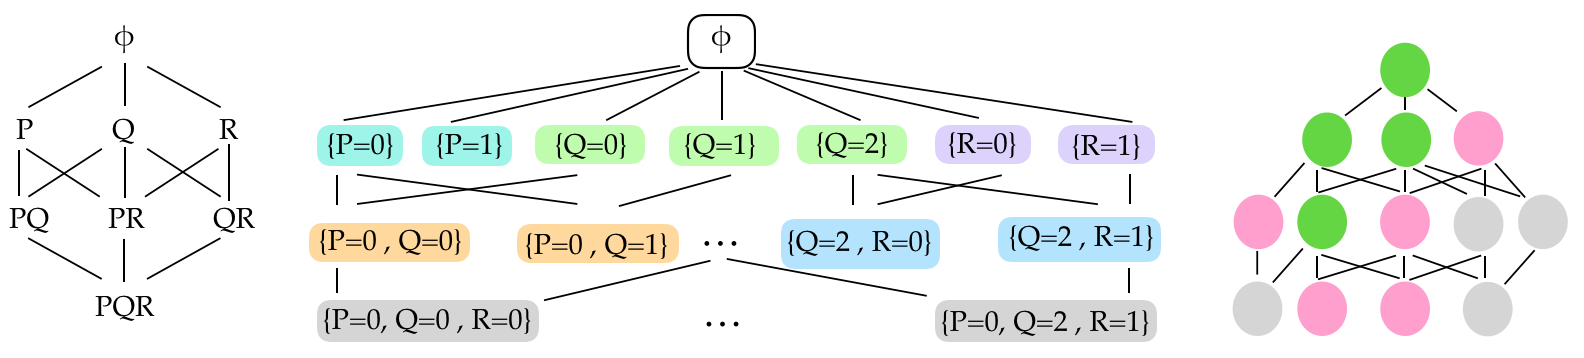
\includegraphics[width=\linewidth]{figures/lattice_frontier.png}
\caption{Left, Middle: Example data subset lattice for a dataset with three binary attributes {\tt \{P, Q, R\}}. The data subsets that belong to the same attribute combinations are highlighted with same color. $\phi$ represents the overall distribution (where no filter conditions is applied). Right: Toy example demonstrating the notion of ``frontier''. Green nodes are selected in the dashboard. The neighbors of the set of selected green nodes are the frontier nodes, shown in pink. Other unpicked nodes in the lattice are shown in gray.}
\label{fig:lattice}
\end{figure*}
We now extend the concept of \emph{containment} for visualizations defined according to our setup.

% \textbf{Viz Containment.} Let $V$ be the set of visualizations (of same type) that show the same $X$ and $Y$ for different $C(Z)$. Given a visualization $V_i \in V$, a parent of $V_i$, $V_i^j$ ($V_i^j\in V$) is a visualization that corresponds to a parent data subset of the former. In Figure~\ref{fig:elections_example} we present three visualizations that show the distribution of votes for 2016 US election candidates in three demographic groups: (i) female voters, (ii) black voters, (iii) black female voters. As per the parent-child relationship among the data subsets, the visualizations corresponding to (i) and (ii) are parents of the visualization corresponding to (iii).

% \begin{figure}[bht]
% \centering
% 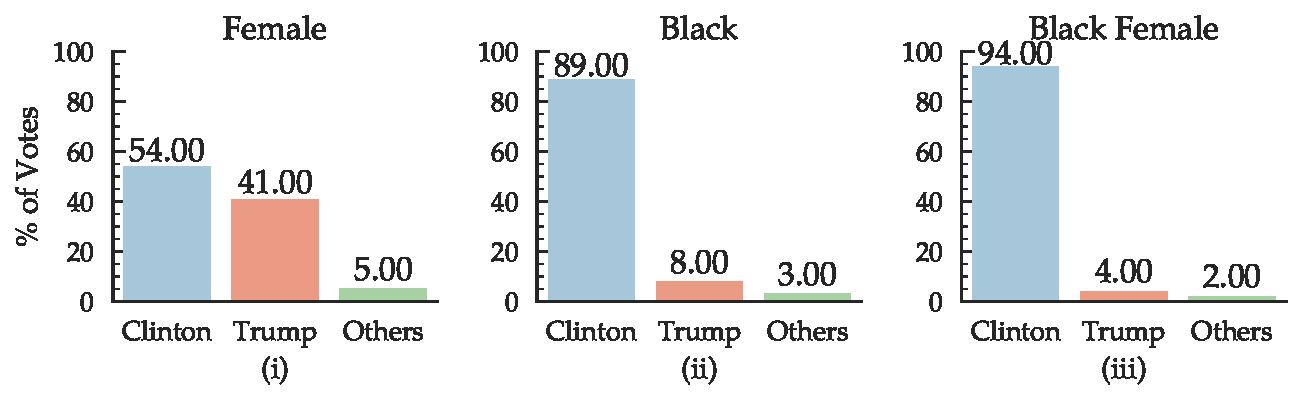
\includegraphics[scale=0.4]{figures/US_Election_Parent_Child.pdf}
% \caption{Parent-child relationship amongst visualizations that show the distribution of votes for 2016 US election candidates in three demographic groups: (i) female voters, (ii) black voters, (iii) black female voters.}
% \label{fig:elections_example}
% \end{figure}

%\haz{Perhaps it will look better if have (iii) in a new line (and centered) to quickly reflect the parent-child relationship.}\dor{Considering that this will take up more space also not sure whether not sure we should mix up the problem formulation with the model itself. Himel?}

% \textbf{Viz Lattice.} Based on the containment relationship of visualizations, we can organize the visualizations from $V$ to form a lattice. This lattice contains all visualizations (of same type, e.g., bar charts) that show the same x- and y- axes for different data subsets, and arranges them as per the parent-child relationships between data subsets. Our goal is to traverse this lattice of visualizations, and identify informative and interesting visualizations.

\subsection{Utility of Visualizations: User Expectation Model\label{sec:utility}}
In order to identify which visualizations should be picked from the lattice, we conduct a formative user study
to study how the presence of one or more of observed parent in the visualization lattice affects an analyst's perception of an unseen visualization. Using these findings, we then model the effective utility of displaying an unseen visualization to a user in the context of seen visualizations.% by defining metrics of \textit{interestingness} and \textit{informativeness}.
%to study how analysts interpret parent-child relationships in a visualizations lattice, and then model the effective utility of displaying an unseen visualization to a user in the context of seen visualizations.
%\textbf{Top Down Traversal.} We observe that, while exploring a dataset, users first look at the top level visualizations before looking at the next level \cite{Kim2017, Hullman2013}. Further, the data distributions learnt from the top level visualizations induce user expectation for the next level. For example, in Example 1, a journalist is likely to examine the voting trends of female or black voters before examining the voting trends of black female voters, and his/her expectation of black female voters would be affected by the observed reference(s) (female or black voters). Based on these two observations, we model user expectation $\hat{V_i}$ corresponding to an unseen visualization $V_i$ based on its seen/observed parents $O(V_i) = \{V_i^1, \ldots, V_i^\lambda\}$ in the visualization lattice.

\stitle{Formative User Study:} %We conducted a user study to understand how a user's perception of an unseen visualization is affected by one or more of its observed parents.
We recruited 9 participants in a study to predict the distribution of an unseen visualization with two constraints. Participants were asked to make a prediction regarding an unseen visualization after seeing the first parent displayed and subsequently after seeing the second parent displayed. For the chosen visualization parents, the first parent have data distributions that very closely follows that of the unseen visualization, whereas the second parent differs greatly from the unseen visualization. In this between-group study, one group of participants (G1) were shown the first parent followed by the second parent, whereas another group of participants (G2) were shown the second parent followed by the first parent. We examined how users form their expectation in presence of these observed parents. The results are summarized in Figure \ref{fig:formative_study}. Our main findings are: (1) participants naturally form their expectations based on one or more observed parents; (2) seeing a parent that well describes the unseen visualization leads participants to better estimate the unseen visualization; (3) in absence of an informative parent, participants can be misled to form an inaccurate expectation; (4) in presence of multiple parents, the variance of expectation increases.
\begin{figure}[h!]
\centering
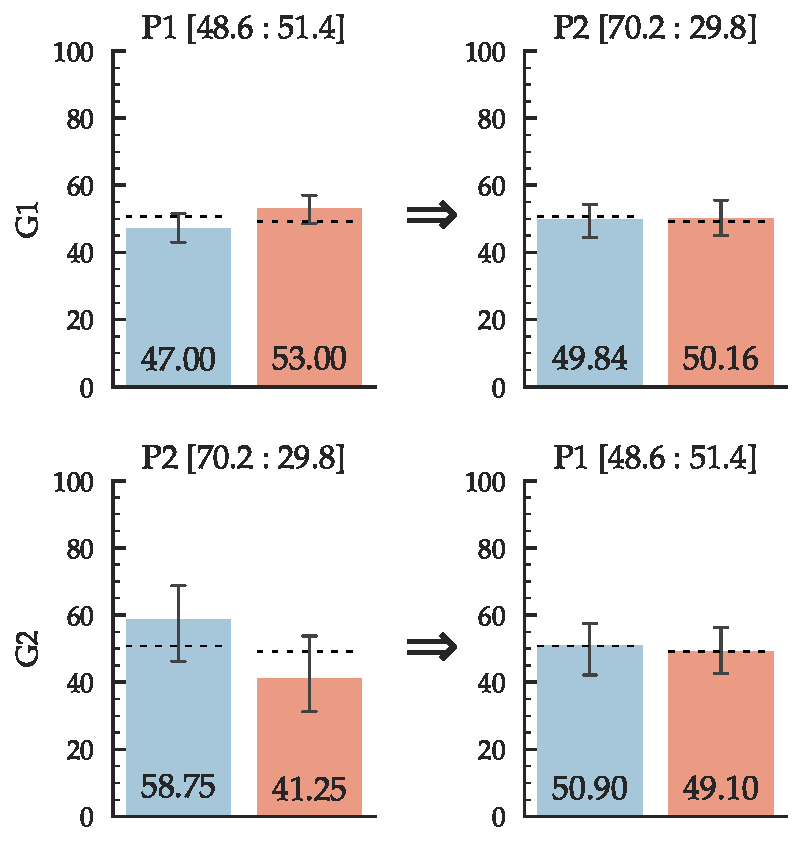
\includegraphics[width=\linewidth]{figures/Formative_Study.pdf}
\caption{Bar charts and error bars showing the mean and variance of participants' estimated distribution during the formative user study. Group 1 (G1) participants were shown the informative parent first, followed by the uninformative parent; whereas Group 2 (G2) participants were shown the uninformative parent first, followed by the informative parent. G1 participants closely approximated the unseen visualization immediately after seeing the informative parent. The ground truth visualization values are shown as dotted lines and printed in square brackets in the visualization title.}
\label{fig:formative_study}
\end{figure}
\npar Based on these findings, we model two aspects of the unseen-visualization and observed-parent relationship through its \textit{interestingness} and \textit{informativeness} criteria.
\stitle{Informativeness:} To model the informativeness of an observed parent in the context of an unseen visualization, we characterize the capability of the parent in predicting the unseen visualization. As highlighted in finding (2), an observed parent is \emph{informative} if its data distribution closely follows the data distribution of the unseen child visualization, since the visualization helps the analyst form an accurate mental picture of what to expect from the unseen visualization. Specifically, we formulate the informativeness of an observed parent $V_i^j$ of an unseen visualization $V_i$ as the similarity between their data distributions measured using a distance function $D(V_i, V_i^j)$. The most informative parents $V_i^*$ of an unseen visualization $V_i$ are the ones whose data distributions are most similar to the unseen.
\begin{equation}
    V_i^*=\underset{V_i^j}{argmin}\ D(V_i, V_i^j)
\end{equation}
Since our finding (4) demonstrates how seeing multiple parents can lead to worser visualization understanding, we allow users to specify a threshold $\theta$ to control the degree of similarity for which a parent can be declared as an informative, such that the distance $D(V_i, V_i^{*, \theta})$ corresponding to the informative parents $V_i^{*, \theta}$ are at least $\theta\%$ close to its most informative parent:
\begin{equation}
    V_i^{*, \theta} = \{V_i^j : \frac{D(V_i, V_i^*)}{D(V_i, V_i^j)} \leq \theta\}
\end{equation}
%Since declaring a parent as informative can vary depending on its similarity with the unseen compared to other parents, we allow the user to specify a threshold $\theta$, which we expect to be close to 1.0, such that the similarity score $S(V_i, V_i^{*, \theta})$ corresponding to the informative parents $V_i^{*, \theta}$ are at least $\theta\%$ of that of the most informative parents'.
For example, if $\theta = 0.8$, all parents of $V_i$ whose similarity scores are at least 80\% of that compared to $V_i^*$ are deemed as \textit{informative}. In Figure~\ref{fig:elections_example}, while both visualization (b) and (d) are considered parents of visualization (h), only visualization (d) (Black) are considered the informative parent of visualization (h) (black female population), for any values of $\theta \geq 11\%$ via the Euclidean distance metric. %the visualization corresponding to black voters is the most informative parent of the visualization corresponding to black female voters. For $\theta <= 0.11$, the former remains the only informative parent of the latter.

\stitle{Interestingness:} While informative parents contribute to the prediction of an unseen visualization, the most interesting visualizations to recommend are those for which \emph{even the informative parents fail to accurately predict the visualization}. \dor{Can we justify this based on our findings?} To model the interestingness of an unseen visualization $V_i$ in the context of an observed parent $V_i^j$, we characterize the deviation between their data distributions using a distance function $D(V_i, V_i^j)$. The unseen visualizations whose data distributions deviate from the observed informative parents are \emph{interesting}. \cut{The most interesting unseen visualizations $V_\#$ are the ones that deviate most from their observed informative parents.
\begin{equation}
    V_\#=\underset{V_i}{argmax} \ D(V_i, V_i^{*, \theta})
\end{equation}
In Figure \ref{fig:elections_example}, the most interesting visualization to recommend is the one corresponding to white female voters. This visualization significantly differs from its informative parent---the visualization corresponding to female voters.} \dor{The argmax notation not necessary since we're just using this in our utility function. The election example is not convincing, the informative parent of white female is actually white and not female. Also the differences are not too significant.}

%\noindent Additional model extensions can be added to this objective function based user specification. For example, there may be $k$ visualizations that approximately yield equal contribution to the user's expectation. For simplicity of notation, we have assumed $k=1$ in the aforementioned model. In order, a user may want to prevent the recommendation of spuriously interesting subsets of the data. We can discard visualizations that falls below a certain subpopulation size threshold.
\stitle{Subpopulation size consideration:} The danger of spurious patterns and correlations in visualizations that contain small subpopulation size is a well-known problem in exploratory analysis~\cite{Binnig2017}. We take two preventive measures to avoid including such misleading visualization in our dashboards. First, in the lattice generation process discussed in Section~\ref{sec:algorithms}, we allow users to select an `iceberg condition' \footnote{The terminology is used in the discussion of iceberg cubes in OLAP literature~\cite{Xin2007}.} ($\delta$) to adjust the extent of pruning on visualizations whose sizes fall below a certain percentage of the overall population size. Second, we downweigh the interestingness edge utility $U(V_i, V_i^j)$ between a parent $V_i^j$ and a child visualization $V_i$ by the ratio of their sizes:
\begin{equation}
    U(V_i, V_i^j) = \frac{|V_i|}{|V_i^{j}|} \cdot D(V_i, V_i^j)
    \label{edge_utility}
\end{equation}
\subsection{Problem Formulation}
Given the lattice data model and the user model for visualization utility described above, the goal of our system is to generate a dashboard by selecting $k$ visualizations from the lattice. We enforce that the generated dashboard satisfies several requirements:
 \begin{enumerate}
 	\item Dashboard must include the overall visualization (topmost visualization with no filter applied) to serve as reference to the rest of the visualizations in the dashboard.
 	\item For each visualization except for the overall, at least one of its informative parents is included within the $k$ visualizations. This excludes the uninformative parents as exemplified in black female example in the dashboard, especially since our findings 3 and 4 shows that showing multiple, improper parents can mislead the participants, resulting in a higher variance across their estimations. %enforces that every visualization shown in

  the dashboard has an informative reference to compare against to create a connected story.
 	\item The selected $k$ visualizations are collectively most ``interesting'' in presence of their informative parents as measured by the utility in Equation \ref{edge_utility}.
\end{enumerate}
 The problem of finding a connected subgraph in the lattice that has the maximum combined edge utility is  known as the maximum-weight connected subgraph problem~\cite{ErnstAlthaus2009} and is known to be NP-Complete, via a reduction from the \textsc{Clique Problem}~\cite{Parameswaran2010}. In Section~\ref{sec:algorithms}, we discuss heuristic algorithms used for deriving a locally optimal solution for ensuring interactive runtime.

%!TEX root = main.tex
\section{System\label{sec:system}}
\subsection{System Architecture}
We have implemented \system\ as a Flask web application on top of a PostgreSQL database. In Figure~\ref{system_architecture}, we present the system architecture of \system, which consists of three core modules: the traversal module, the query module, and the statistics module. The interaction manager deals with the supported user interaction described in Section~\ref{sec:interaction} and sends a request to the lattice module which  contains several algorithms for generating and traversing the visualization lattice described in Section~\ref{sec:algorithms}. For generating the visualization lattice, the lattice module passes a list of data subsets corresponding to visualizations to be generated to the query module. The query module translates these visualizations into queries, and then optimizes (by grouping) and executes the queries. The statistics module is an optional module that allows the lattice module to prune low-utility visualizations without actually generating them. Specifically, it generates coarse statistics for the unexplored visualizations based on the current list of explored visualizations. Finally, the dashboard renderer takes the resulting visualizations to be included in the dashboard and perform any rendering preprocessing procedures for display and navigation of the dashboard as described in Section \ref{sec:navigation}.
\begin{figure}[ht!]
\centering
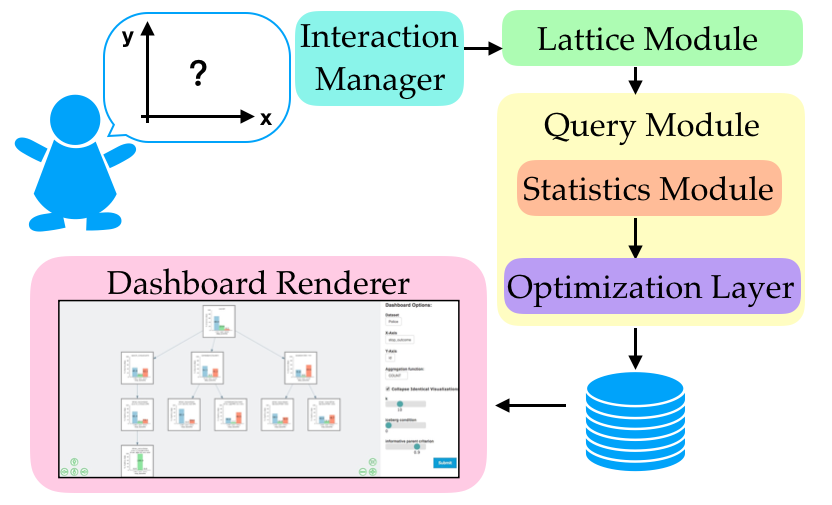
\includegraphics[width=\linewidth]{figures/system_architecture.png}
\caption{System Architecture of \system. User starts with x and y axes of interest and requests for $k$ visualizations in the dashboard. The request is processed by generating the lattice with the help of the querying module, visualization selection through the lattice traversal algorithms, and finally the dashboard is displayed at the frontend through the dashboard renderer. }%  The interaction manager translates the request to the traversal module that ???? [should we look at the offline case??]}
\label{system_architecture}
\end{figure}

\subsection{Algorithms\label{sec:algorithms}}
We give an overview of our algorithms by first discussing the approaches to generate the visualization lattice, and then presenting a high-level overview of our traversal algorithms.

\stitle{Lattice Generation.} Our system supports two variants of traversal algorithms based on the lattice generation procedure---offline variants that first generate the complete lattice and then work towards identifying the maximum utility solution, and online variants that incrementally generate the lattice and simultaneously identify the solution. The offline variants are appropriate for datasets with a small number of low-cardinality attributes, where we can generate the entire lattice in a reasonable time; whereas the online variants are appropriate for datasets with large number of high-cardinality attributes, where we incrementally generate a partial lattice.

%In most cases, the lattice contains a large number of visualizations due to the presence of many attributes or high-cardinality attributes in the dataset. In such cases finding an optimal solution is computationally challenging.

\stitle{Lattice Traversal.} Given the materialized lattice, the objective of the traversal algorithm is to find the connected subgraph in the lattice that has the maximum combined edge utility. Here, we discuss the \textit{frontier greedy} algorithm which is used for generating the dashboards for our user study and defer our discussion on the details of other algorithms that we have developed to the technical report.
% \begin{figure}[ht!]
% \centering
% 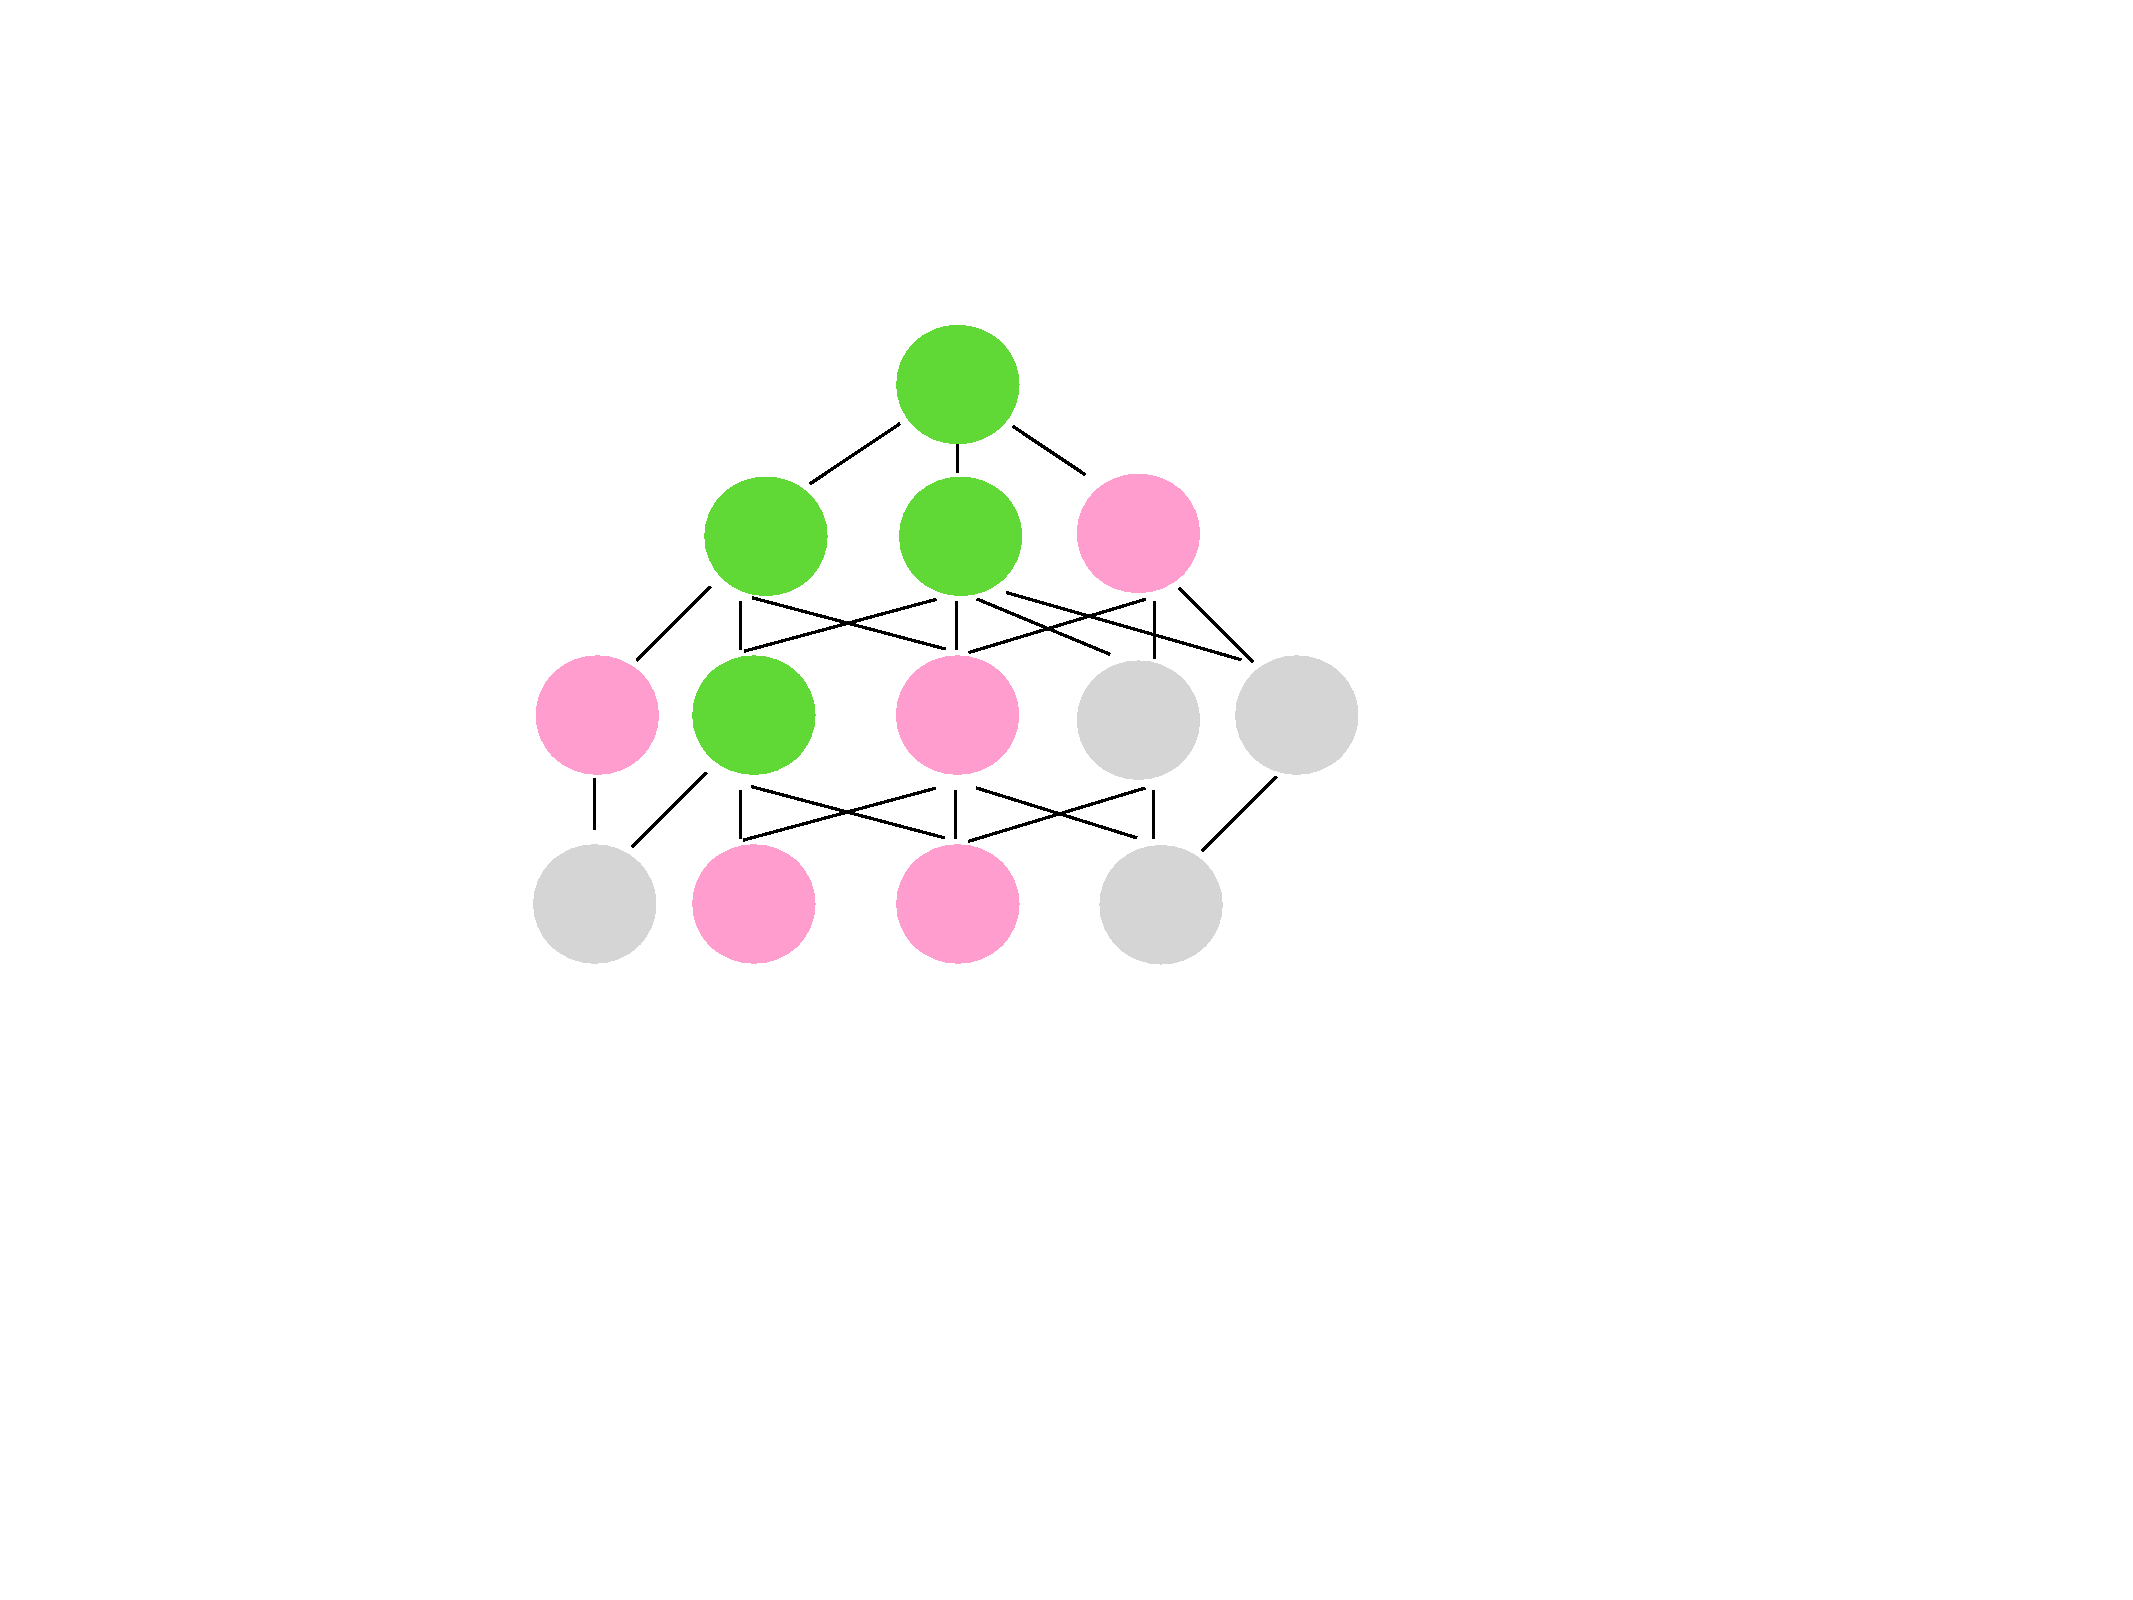
\includegraphics[width=0.4\linewidth]{figures/frontier.pdf}
% \caption{Toy example demonstrating the notion of ``frontier''. Nodes that have been picked to include in the dashboard are colored green. The neighbors of the set of picked nodes are the frontier nodes, shown in pink. Grey nodes are other unpicked nodes in the lattice.}
% \end{figure}
%We devised two classes of heuristics algorithms, namely, frontier-based algorithms, and path-merging algorithms. These algorithms are guaranteed to find a solution that satisfies the constraints of our problem, except for the optimality.
\techreport{The frontier-based algorithms traverse the lattice from root to downwards, incrementally adding new nodes (visualizations) to the current solution (dashboard) till it reaches the maximum capacity $k$. To achieve this, the algorithms maintain a list of candidate nodes---called \textit{frontier} nodes---any of which can be added to the current solution since their informative parent is already present in the solution. At each step, the algorithms add a node from frontier to the current solution, and update the frontier accordingly.  The frontier based algorithms can be further categorized into three types based on their node selection strategy (from frontier), namely greedy algorithm, random walk algorithm, and probabilistic algorithm. The greedy algorithm picks the current best node from frontier (thus concentrates on exploitation), random walk algorithm picks a random node (thus concentrates on exploration), and probabilistic algorithm picks a random high-utility node (thus trades off between exploration and exploitation).}
\par As described in Algorithm \ref{algo:frontier_greedy}, our algorithm obtains a list of candidate nodes known as the \textit{frontier} nodes (pink in Figure\ref{fig:lattice} left), which encompasses all neighbors of nodes in the existing subgraph solution. Any of the nodes in the frontier can be added to the current solution since their informative parent is guaranteed to be present in the solution. The \texttt{getFrontier} function scans and adds all children of leaf nodes of the current dashboard as part of the frontier. In the online version, it additionally checks for each child whether its informative parent is present in the current dashboard. At each step, our algorithm greedily picks the node with the maximum utility from the frontier to the current solution, and updates the frontier accordingly.

\techreport{The path merging algorithm first generate the informative paths from root to every candidate node. Then, it greedily merges the paths with high-utility to create a subgraph whose size is less than or equal to maximum capacity $k$.}

% \begin{algorithm}
%     \SetKwInOut{Input}{Input}
%     \SetKwInOut{Output}{Output}
%     \Input{Precomputed Lattice of Visualizations, $G = \{V_1, \ldots, V_n\}$}
%     \Output{A Dashboard of Size $k$, $S$}
%     $S = \{ V_{root}\}$\;
%     $F = get\_child(V_{root})$\;
%     \While{$size(S) < k$}
%     {
%     	$s_{next} = pick\_next(F)$\;
%     	$S = S \cup s_{next}$\;
%       \For{$i = 0;\ i < size(S);\ i = i + 1$}
%       {
%           $F = (F \cup get\_child(S[i])) - S$\;
%       }
%     }
%     return $S$\;
%     \caption{Frontier Based Algorithm}
% \end{algorithm}

\begin{algorithm}
  \begin{algorithmic}[1]
  \Procedure{pickVisualizations}{k,lattice}
  \State dashboard $\gets$ \{ $V_{overall}$ \}
  \While{|dashboard| < k}
      \State frontier $\gets$ getFrontier(dashboard,lattice)
      \State maxNode $\gets$ getMaxUtilityNode(frontier)
      \State dashboard $\gets$ dashboard $\cap$ \{maxNode\}
  \EndWhile
  \Return dashboard
  \EndProcedure
  \end{algorithmic}
  \caption{Frontier Greedy Algorithm}\label{algo:frontier_greedy}
\end{algorithm}

%\textbf{Greedy Algorithms:} Greedy algorithms select the locally optimal node to be added to the frontier.

%A specific implementation would need to specify a scoring function to nodes in frontier that is used to pop out the next node in each iteration. One can design a scoring function based on the trade-off between performance and complexity. In the most simple case, we can use the edge weights to score nodes in the frontier. That is, at each point we add a node with the highest interestingness value. We note that this is quite a greedy approach. Specifically, we might miss visualizations with high utility that are in deeper levels of the graph. Thus, another approach would be to extent the horizon for which we calculate a nodes utility. We denote such approach as a look-ahead approach. With a free parameter $n$, we would like to assign a score to each frontier node the corresponds to the expected utility of adding this node and $n-1$ more nodes who are its descendants. For example, we can run BFP for each node in frontier treating it as a root.

\techreport{The path merging algorithm first generate the informative paths from root to every candidate node. Then, it greedily merges the paths with high-utility to create a subgraph whose size is less than or equal to maximum capacity $k$.}

\section{User Interaction\label{sec:interaction}}
\begin{figure}[ht!]
\centering
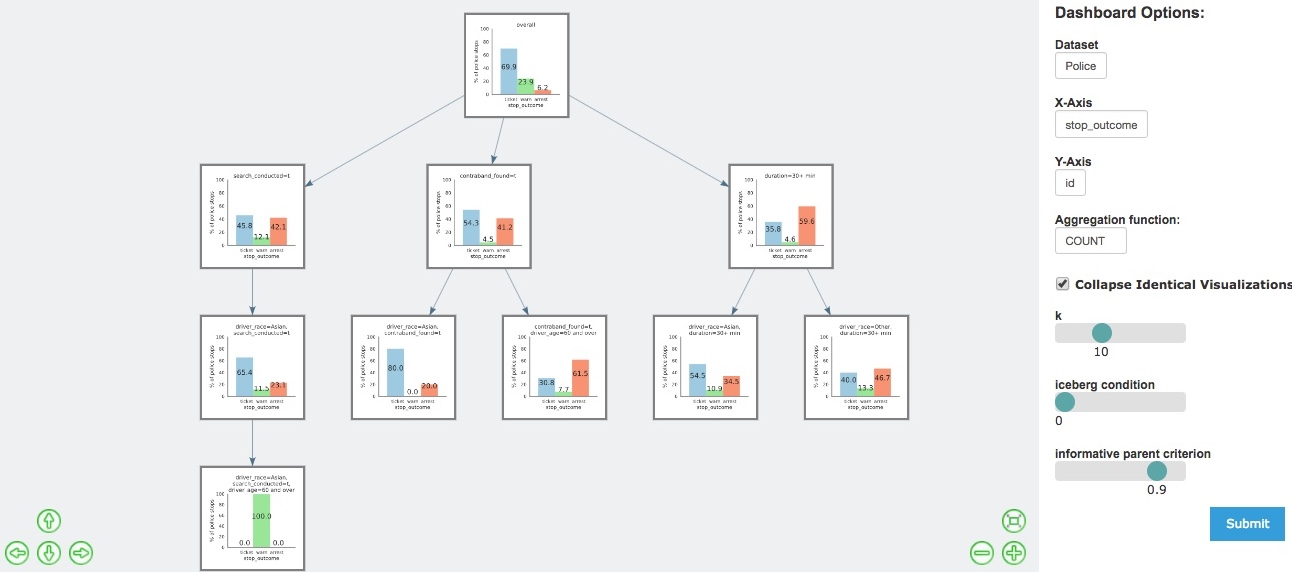
\includegraphics[width=\linewidth]{figures/overview.jpeg}
\caption{Overview of the \system interface for the Police Dataset. Users can select x and y axes of interest, as well as a choice of an aggregation function. Default values are set for system related parameters such as the number of visualizations to show in the dashboard (k), iceberg condition for pruning ($\delta$), and informative parent criterion ($\theta$), which can be adjusted by the users via the sliders if needed.}
\label{fig:overview}
\end{figure}
\par Figure \ref{fig:overview} shows an overview of the \system interface. After the user selects the x and y axes of interest, aggregation function, and optional system parameter settings, an initial dashboard of $k$ visualizations is displayed on the canvas, such as the one seen in main canvas of Figure \ref{fig:overview}.  The system provides toolbar buttons with keyboard binding for zooming in, out, and extent, as well as moving around the canvas. Alternatively, users can zoom and pan with mouse click and scroll.

%\hdev{(1) The second sentence is in passive voice. (2) What are the optional system parameters? Clearly state them. (1) Simplify the third sentence. A non-UI person may not know the meaning of some of the terms. (1) In fourth sentence, if you are using "alternatively", there's no need for "also".}

\par After browsing through the visualizations in the dashboard, users may be interested in getting more information about a particular node. \system supports a mechanism for users to request additional summarizations based on a chosen visualization of interest. As shown in Figure \ref{fig:altroot_expansion} (left), the analyst starts with a 5-visualization dashboard. He learns that for the drivers who had contraband found in the vehicle, the arrest rate for drivers who are 60 and over is surprisingly higher than usual, whereas for Asian drivers the arrest rate is lower. In addition, he is also interested in learning more about the other factor that contribute to high arrest rate: duration=30+min. He clicks on the corresponding visualization and requests for 2 additional visualizations. Upon seeing the updated dashboard in Figure~\ref{fig:altroot_expansion} (right), he learns that similar to the selected visualization, any visualizations that involves the duration=30+min filter results in high ticketing and arrest rates. This implies that if a police stop last more than 30 minutes, the outcome would more or less be the same, independent of other factors, such as driver's race or age. \system uses the same models and algorithms as before, except the root node is now set as the selected visualization, rather than the overall visualization. This node expansion capability is similarly motivated by the idea of \textit{iterative view refinement} in other visual analytics system \cite{Wongsuphasawat2016,Hoque2017}, which is essential for the users to iterate on and explore different hypotheses.

\begin{figure}[ht!]
\centering
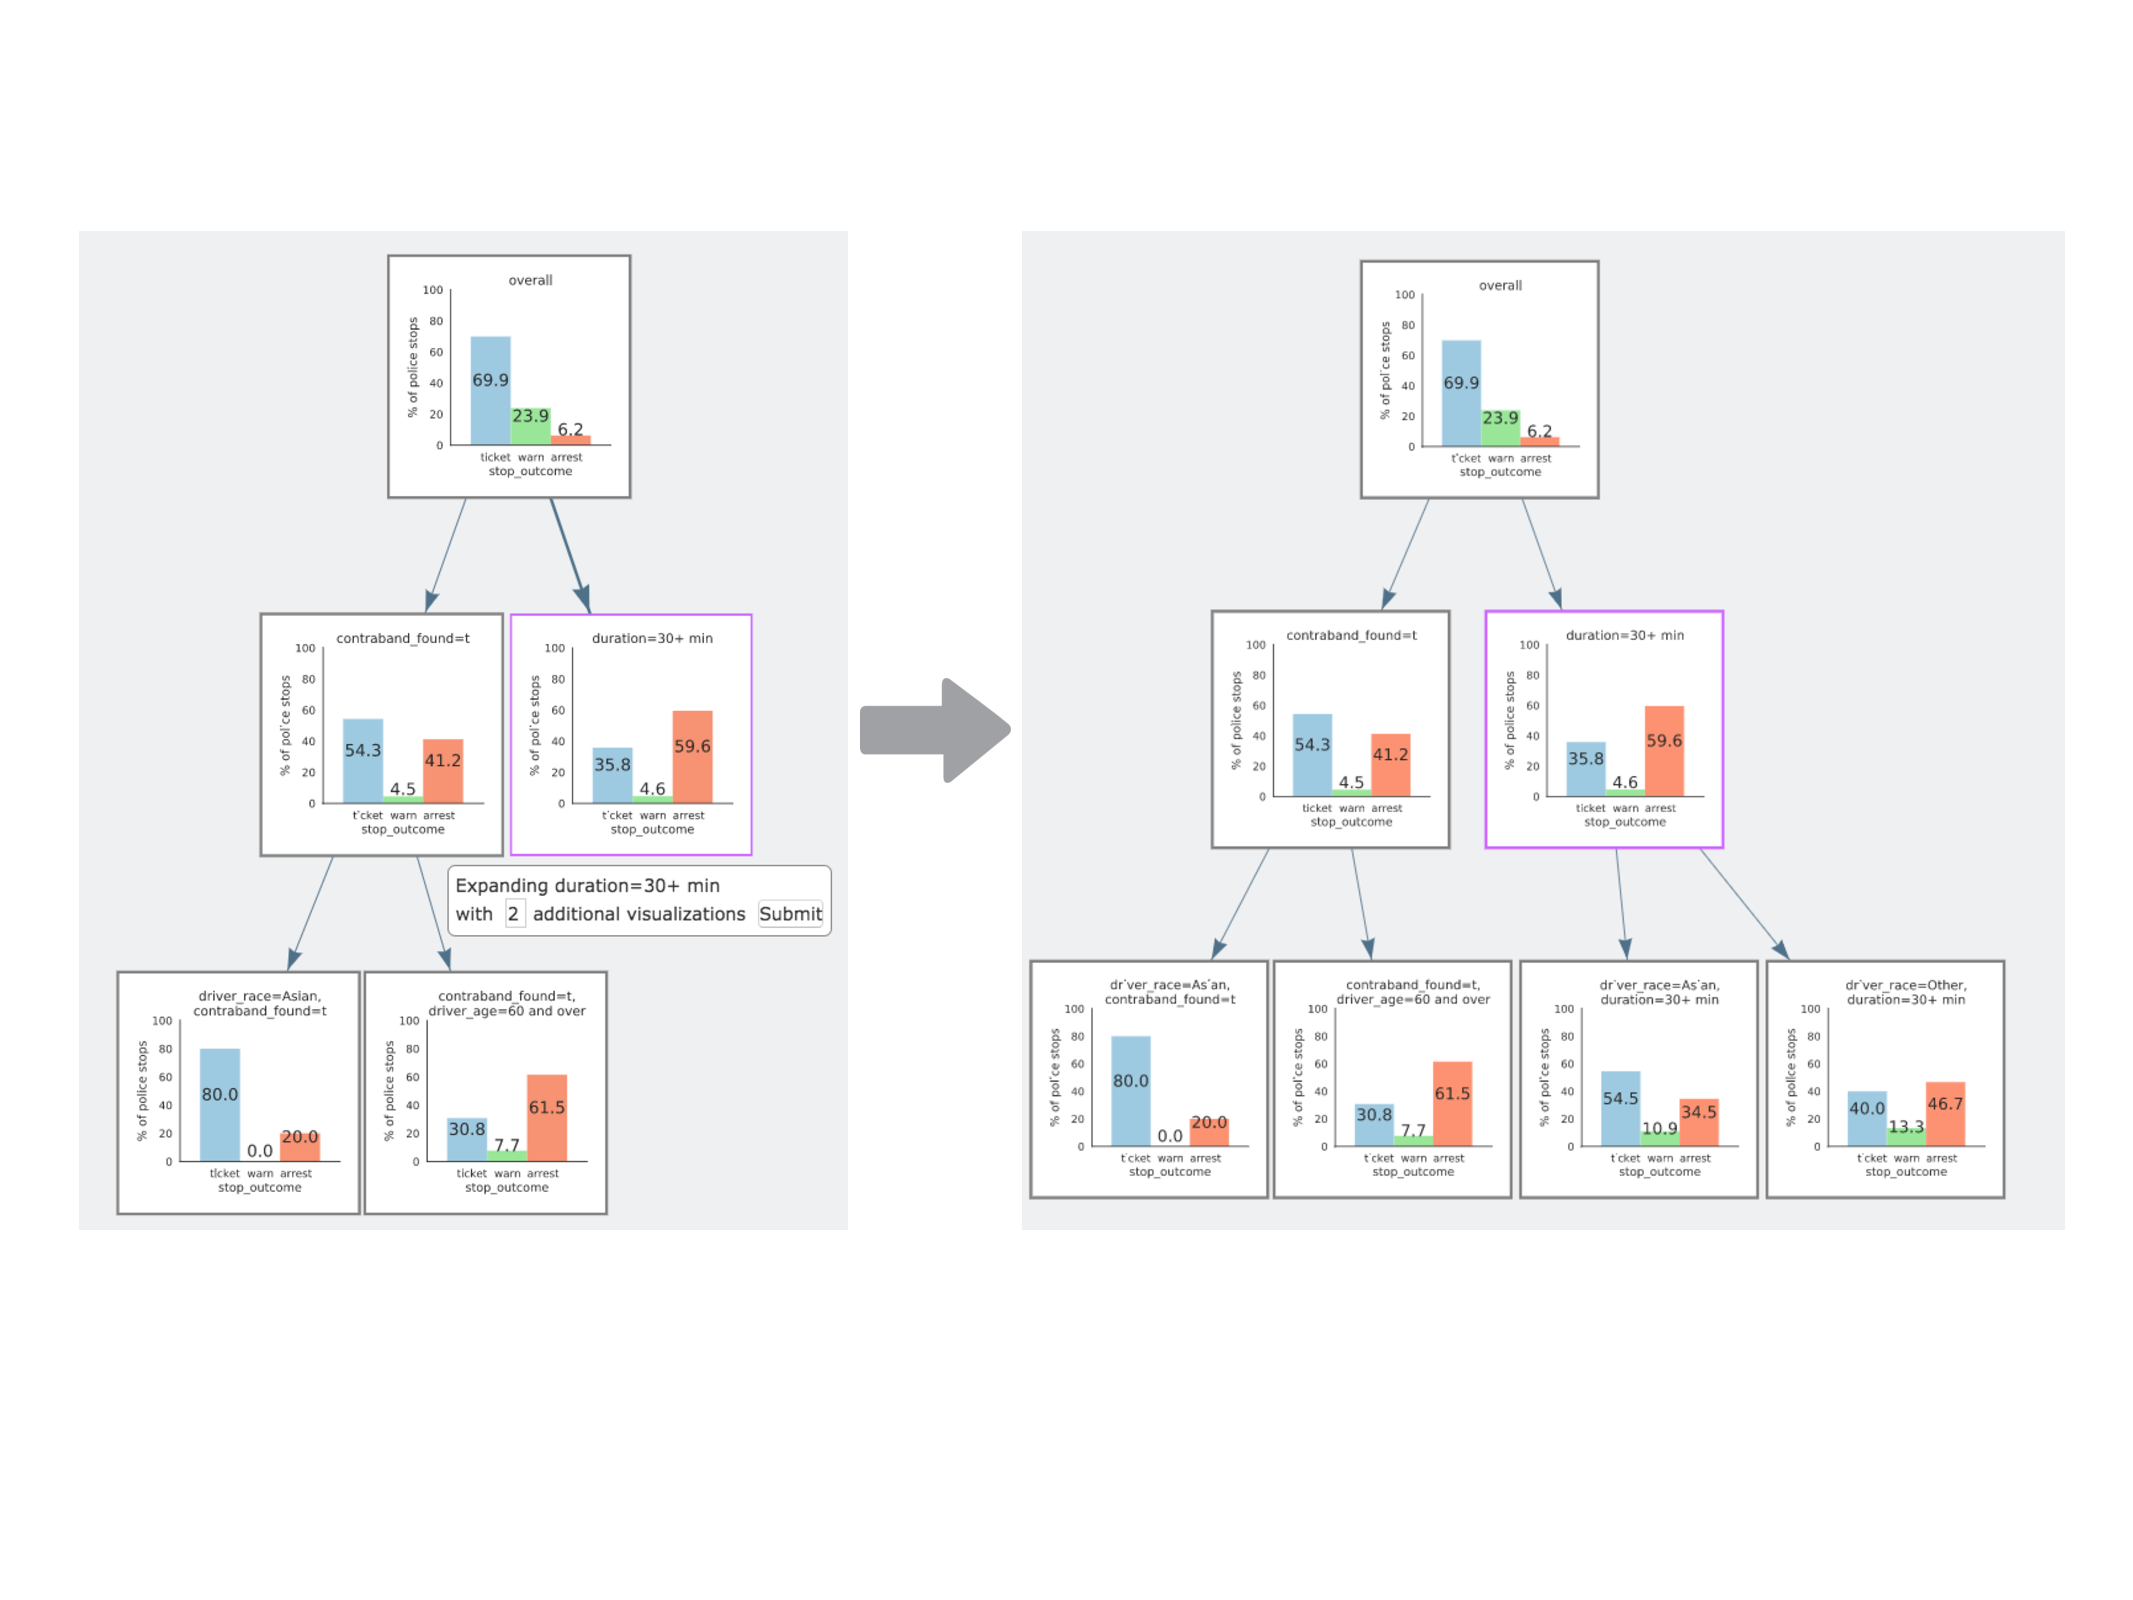
\includegraphics[width=\linewidth]{figures/expansion_example.pdf}
\caption{Left: Original k=5 dashboard with the duration=30+min visualization clicked. A pop-up is displayed to submit the request for additional summary visualizations to be generated. Right: Resulting dashboard after requesting for 2 more visualizations based on the visualization of interest.}
\label{fig:altroot_expansion}
\end{figure}

\subsection{Assistive tools for visualizing large lattices\label{sec:navigation}}
Due to the amount of space occupied by the hierarchical layout when the number of visualizations gets large, we have developed tools to help users navigate through different parts of the dashboard interactively.
\stitle{Navigation Minimap:}  When the user zooms in on the dashboard, an overview mini-map is shown on the upper right-hand side of the canvas to help users identify which region of the dashboard they are currently exploring, as shown in Figure \ref{fig:hover_minimap}.
\stitle{Collapsed visualizations:}
One observation that we found across several datasets was that many visualizations had identical distributions, which resulted in lots of wasted space. Apart from their attribute name, these visualizations are not very informative for the users, therefore, we offer an option to collapse these visualization, as demonstrated in Figure \ref{fig:collapse_demo}. A visualization can be collapsed if it has more than one redundant sibling and does not have any children, so that there are no hidden stories due to lower-level dependencies. As shown in Figure \ref{fig:hover_minimap}, collapsed nodes can be easily identified by an orange border and the details of which visualizations are in the collapsed node are displayed when the user hovers over the visualization.
%\afterpage{%to enable footnote in caption
\begin{figure}[ht!]
\centering
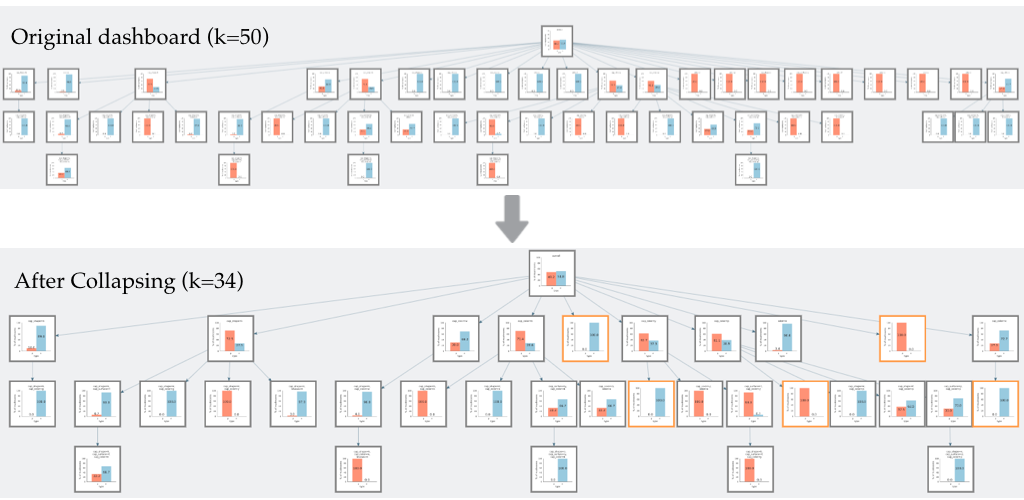
\includegraphics[width=\linewidth]{figures/collapsed_example.png}
\caption{An example of the k=50 dashboard for the mushroom dataset\cite{mushroom}, which contains type=\{posionous, edible\} on the x-axis. The collapsed dashboard (bottom) removed 16 redundant visualizations from the original dashboard (top).}
\label{fig:collapse_demo}
\end{figure}
%}
\begin{figure}[ht!]
\centering
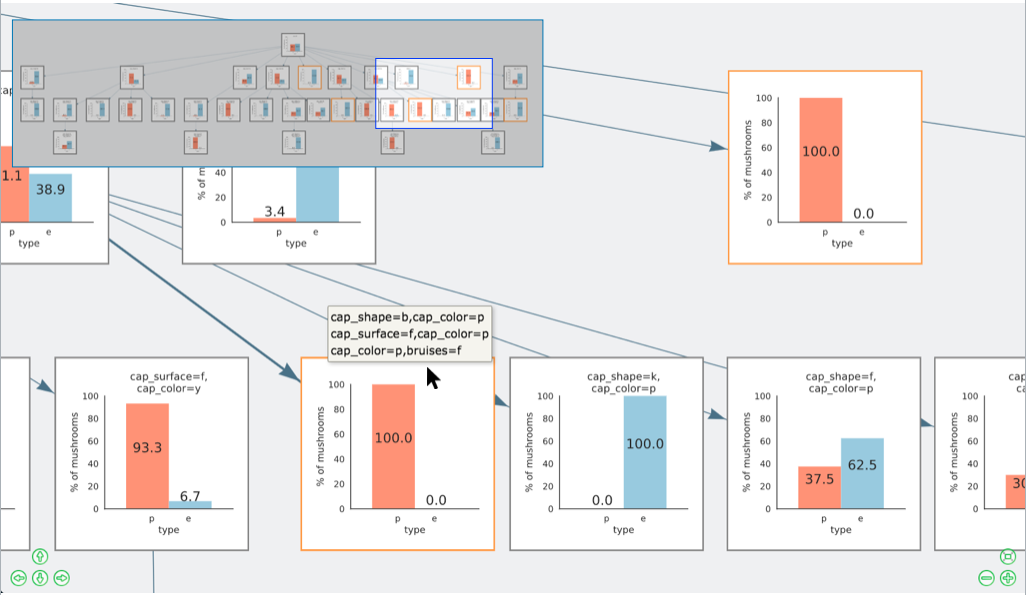
\includegraphics[width=\linewidth]{figures/minimap_zoom.png}
\caption{Zoomed-in version of Figure \ref{fig:collapse_demo} showing the labels of a collapsed visualization when user hovers over the visualization. The navigation minimap is shown in the top-left to help users navigate through the large dashboard.}
\label{fig:hover_minimap}
\end{figure}

%!TEX root = main.tex
\section{User Study Evaluation\label{sec:userstudy}}
\subsection{Procedure}
Given that our formative study motivated our metrics and constraints used in the problem formulation, we further evaluate the utility of our tool by performing a user study focusing on addressing the research questions:
\begin{denselist}
	\item RQ1: How effective is our tool at discovering key insights within a given dataset?
	\item RQ2: How effective is our tool in providing analysts with task-specific insights? (including identifying important features for prediction tasks and estimating the distribution of an unseen visualization)
	\item RQ3: How useful are the visualizations in the recommended dashboard to analysts?
\end{denselist}

We recruited 18 participants who have prior experience working with data. Participants include undergraduate and graduate students, researchers, and data scientists, with 1 to 14 years of data analysis experience (average = 5.61).  %This can include, but are not limited to, browsing and reading data, data cleaning and wrangling, data visualization and model building. The inclusion criteria is assessed based on a self-reporting basis in the pre-study survey.
%an average of 5.61 years of experience working with data.
There were 8 female participants and 10 male participants. No participants reported prior experience in working with the two datasets used in the study.

\par In this between-group study, participants are randomly assigned two of the three following conditions.
\begin{enumerate}
	\item \system: The dashboards for this condition is generated by the frontier greedy algorithm (described in Section \ref{sec:algorithms}) and displayed in a hierarchical layout (as seen in Figure~\ref{fig:overview}). In order to establish a fair comparison with the two other conditions, we deactivated the interactive node expansion and dashboard navigation functionalities described in Section \ref{sec:interaction}, especially since the k=10 dashboard was small enough to function without the navigation tools.

	\item \cluster: K-Means clustering is performed on the dataset with $k$ clusters, corresponding to $k$, the number of visualizations to be shown in the dashboard. For each representative cluster, we select the visualization that has the least number of filter conditions for interpretability\footnote{Due to this requirement, the overall visualization is guaranteed to be picked as one of the displayed visualizations.} and display them in a 5x2 table layout.

	\item \BFS: Starting from the overall visualization, $k$ visualizations is selected in level-wise order: sequentially adding visualizations at the first level with 1-filter combination one at a time, proceeding with the 2-, 3-, etc. filter combinations, until $k$ visualizations have been added to the dashboard. This baseline is designed to simulate the dashboard generated by a meticulous analyst who has generated all possible visualization combinations to display on a visualization dashboard and is scrolling through the dashboard to browse and inspecting every visualization. The chosen visualizations are displayed in a 5x2 table layout in the traversed order.
\end{enumerate}
All generated dashboards had k=10 visualizations. We randomize the ordering for each task combination to prevent confounding learning effects.
\par The study begins with a 5 minute tutorial using dashboards generated for the Titanic dataset. To prevent participant's bias, participants were not provided an explanation of how the dashboard is generated and why the visualizations were arranged in a particular way. Then, participants proceeded onto the Police dataset\cite{police} %, which contains visualizations of the \% of police stop that resulted in a warning, ticket, or an arrest.
, which contains a total of 312948 records of vehicle and pedestrian stops from law enforcement departments in Connecticut, dated from 2013 to 2015. We generate a dashboard of visualizations with bar charts with x-axis as the stop outcome (whether the police stop resulted in a ticket, warning, or arrest/summons) and y-axis as the percentage of police stops that led to this outcome. The attributes in the dataset include driver gender, age, race, and the stop time of day, whether a search was conducted, and whether contraband was found.
\par Participants were given some time to read through a worksheet containing descriptions of the data attributes. Participants were given an attention check question where they are asked to find and read off the values of a visualization in the dashboard. In the main experiment, participants were asked to accomplish the following tasks in the prescribed order below:
\agp{why were these selected?}\dor{I reserved the discussion of why these task were selected to the results and discussion section, since they make more sense in the context on the results. I thought the methods section usually reads more like a recipe.}

\stitle{Retrieval:} Participants were asked to talk aloud as they interpret the visualizations in the dashboard and mark each visualization as either interesting, not interesting, or leave it as unselected.

\stitle{Attribute Ranking:} Participants were given a worksheet with all the attributes listed and asked to rank the attribute in order of importance in contributing to one particular x-axis value (e.g. stop outcome = arrest, autism = yes)

\stitle{Shallow Prediction:} Participants were given a separate worksheet and asked to draw an estimate for a visualization that is not present in the dashboard. The visualization to be estimated is ``shallow'' in the sense that it is a visualization with 2 filter combinations, with one parent present in the given dashboard. After making the prediction, participants are shown the actual data distribution and asked to rate on a Likert scale of 10 how surprising was the result.

\stitle{Deep Prediction:} Similar to the shallow prediction, except that the visualization to be estimated is ``deep'' in the sense that it is a 3-combination filter, with only one parent in the given dashboard.

\par The second dataset in the study is the Autism dataset\cite{autism}, which includes the result of autism spectrum disorder screening for 704 adults. The attributes in the dataset are  binary responses to 10 questions that are part of the screening process. Participants are not given the descriptions of the questions nor the answers corresponding to the labels. We generate dashboard visualizations based on whether the participant is diagnosed with autism or not. We repeat the same procedure described above for the Autism dataset. At the end of the study, we asked two open-ended questions regarding the stories and insights that they have learned and what they like or dislike about each dashboard.
%The user study is composed of two phases. Phase one of the experiment focuses on comparing our tool against a set of baselines intended to simulate the natural sequence of visualizations that an analyst would encounter through various approaches during exploratory analysis. The baselines include:
%To prevent learning effects, the ordering of the baselines will be randomized across users.
% \par At the beginning of the study, participants were provided with a dashboard from an example dataset, as well as an explanation of how the dashboard is generated. For each of the visualization dashboard, participants are asked to mark visualizations as interesting/not interesting while explaining their reasoning for each annotation. Then, they are asked to summarize a list of insights that they have discovered after browsing through all visualizations in the dashboard. Participants also answer a set of task-specific questions related to causality and outliers[?], in the form as shown in the example [*]. These tasks are repeated for all baselines and our tool in randomized order on different datasets to prevent learning effects. At the end of phase one, participants are asked to comment on their experiences with each method, as well as the pros and cons of each of the tools. This phase of the experiment is designed to quantify the effects of RQ 1 and 2. In the end, we ask participants to discuss the interesting insights drawn from looking at the recommended dashboards as well as  ------.
%\par To prevent fatigue, after a 5 minute break, the participants then proceed onto phase two of the study, where they are given [10] dashboards generated by our tool and are asked to engage in a talk-aloud exercise as they browse the recommended visualizations. This is a more open-ended study intended for addressing RQ3 that can reveal our tool show unimportant results across different datasets and/or highlight larger selection of the types of insights that can be generated from the tool.
\subsection{Results}
In order to evaluate the efficacy of our system against the two baselines, we will first examine the quantitative results to address RQ1 and RQ2 and then discuss the qualitative findings to address RQ3.
\dor{In general, we might have to make better connection between the RQs and the study results.}
\stitle{Retrieval (RQ1):} Using the click-stream data logged from the user study, we record whether each user is interested, not interested, or have not selected a visualization in the dashboard. %Since we do not have objective ground truths of which visualization is interesting or not, we use the participant's consensus to come up with a score for each visualization. In this scoring scheme, if visualization is marked as interesting, that visualization receives a score of 1; if a visualization is marked as uninteresting, the visualization incurs a penalty of -0.5\footnote{The reason why we chose a lower penalty score for disinterested clicks than the interested click reward is that some of the participants did not chose to mark visualizations that they thought were uninteresting as disinterested explicitly and chose to simply keep them unselected.}; no score is assigned if the visualization is unselected, then the scores are summed over all users who have seen the visualization. Each user is then assigned a score based on the product of their retrieval score and the consensus score (i.e. user would receive a higher score if selected visualization was highly ranked by consensus).
Since we do not have a objective ground truth on which visualization is interesting or not interesting, we devise a voting-based measure that measures how interesting is a visualization amongst all participants. Here i indexes the visualization and j indexes the user. As shown in Equation~\ref{weighting}, we assign a vote $\delta_{ij}$ of 1 if a user is interested in a visualization, 0 if they leave it unselected, and -1 if they are not interested in a visualization.
\begin{equation}\label{weighting}
	\delta_{ij}= \left\{\begin{matrix}
	 1& \textrm{interested}
	\\ 0 & \textrm{unselected}
	\\ -1 & \textrm{not interested}
	\end{matrix}\right.
\end{equation}
We obtain a consensus score for each visualization to measure how frequently the visualization is regarded as interesting by summing over all user's vote on that visualization.
\begin{equation}\label{vote}
\textrm{consensus}(V_i) =\sum_{j\in user} \delta_{ij}
\end{equation}
Given a consensus measure of how interesting a visualization is, we can define a rating score which measures how good a particular user's rating is, by taking the product of the consensus interestingness score and the rating value, as shown in Equation \ref{rank}. Intuitively, a rating should be rewarded more if it has retrieved interesting visualization agreed by many other users, likewise, ratings that does not retrieve such visualizations should be penalized more heavily.
% describes how the rating score (which measures how good the user's particular rating is) is the product of consensus score (how frequently is a visualization regarded as interesting?) and the rated value ($\delta_{ij}$).
\begin{equation}\label{rank}
\textrm{rating score}(V_{ij}) =votes(V_i) \cdot \delta_{ij}
\end{equation}
Table~\ref{table:interestingScore} summarizes results of rating scores averaged over the tasks that the user performed.
\begin{table}[ht!]
	\centering
	\begin{tabular}{lrrr}
		\hline
		 Dataset   &   \system &   \cluster &   \BFS \\
		\hline
		 Police    &        62 &        52 &    99 \\
		 Autism    &       213 &       180 &   114 \\
		\hline
	\end{tabular}
	\caption{Average consensus-agreement score for different algorithm and datasets.}%\agp{breakdown by interested and not interested}}
	\label{table:interestingScore}
\end{table}
%Even though participants were asked to --- daily experiences to answer the question, b
\npar Due to the highly subjective nature of the retrieval task, the interestingness selection for the Police dataset was biased by participant's priors and intuition about the attributes. For example, while all participants who have seen the visualization "duration=30+min" verbally noted that stop duration is a crucial factor that leads to arrest, only 4 users marked it as interesting. 5 participants marked the visualization as not interesting and 4 left it unselected, because the visualization was not very surprising as it agreed with their intuition that ``\textit{if the police stop is taking a long time, something has probably gone wrong}''.
\par Since the attributes in the Autism dataset are simply question numbers, participants could not associate any priors to their interestingness selection. In this prior-agnostic case, participants who used \system\ found more visualizations of interest that corresponded to the consensus, indicating that there are more interesting visualizations picked out by \system\ than compared to the two baseline-generated dashboards.

\stitle{Attribute Ranking (RQ2):}
To determine attribute importance ranking for a dataset, we computed the Cramer's V statistics between attributes to be ranked and the attributes of interest. Cramer's V test makes use of the chi-square statistics to determine the strength of association between attributes. Using the ranks determined by Cramer's V as ground truth, we compute the normalized discounted cumulative gain (NDCG@k) of each participant's ranking average over all tasks\footnote{Since participants are asked to examine all attributes, the k for NDCG@k corresponds to total number of attributes in that dataset.}, as detailed in Table \ref{table:ndcgRankingResult}.
\begin{table}[ht!]
	\centering
	\begin{tabular}{lrrr}
	\hline
	 Dataset   &   \system &   \cluster &   \BFS \\
	\hline
	 Police    &      0.63 &      0.45 &  0.84 \\
	 Autism    &      0.50 &      0.30 &  0.24 \\
	\hline
	\label{table:ndcg_ranking_result}
	\end{tabular}
	\caption{NDCG@10 scores for the attribute ranking task.}
	\vspace{-10pt}
    \label{table:ndcgRankingResult}
\end{table}
We see that \system\ performs better than clustering in both cases. Since clustering seeks for a set of visualization that exhibits diversity in the shape of the data distribution, it results in visualizations with many filter combination, which is hard to interpret without appropriate context to compare against. \BFS performs better than \system in the Police dataset, but not in the Autism dataset. \BFS may have performed better than \system\ in the Police dataset for a combination of two reasons: 1) since \BFS exhaustively displays all attributes sequentially, for the Police dataset it had happened to select several of the important attributes (related to contraband and search) to display as the first 10 visualizations and 2) as discussed earlier, some participants had priors on the data attribute which influenced their ranking. However, with a budget of k=10, only visualizations regarding questions 1-5 fit in the dashboard for the Autism dataset, so the poor ranking behavior comes from the fact that the \BFS generated dashboard failed to display the important attributes (questions 6 and 9) given the limited budget.
\npar Attribute ranking tasks are common in feature selection and other data science tasks, in general, our results indicate that using \system, users gain a better understanding of variable influence and correlation.

\stitle{Prediction (RQ2):} In order to measure how accurate participants' decisions are, we computed the Euclidean distance between their predicted distributions and ground truth data distributions. As shown in Figure \ref{fig:distance} (top), all the shallow predictions made by using information from the \system\ is closer to the actual distribution compared to the baselines. This aligns with our findings in the formative study and indicates that users are able to more accurately reason about how unseen data would behave with \system.
\par \system\ did not perform as well compared to the baselines for the Autism deep prediction task. One possible reason for this is due to the fact that the shallow and deep prediction tasks for the Autism dataset were correlated. Therefore, after learning about the insights that answering 1 on question 9 results in a very high probability for an autism diagnosis, some participants made use of that information when tackling the subsequent deep prediction task. By discussing with the baseline participants on how they have obtained the prediction estimates, they described how surprised they were by the finding in the shallow prediction and therefore adjusted the autism diagnosed values to be higher to compensate for their mistake in the subsequent deep prediction task.
\par As shown in Figure\ref{fig:distance} (bottom), in general, we find that participants who used \system\ reported that they were less surprised when the unseen visualization is revealed, which again indicates that participants had a more accurate mental model of prediction.
\par We also compute the mean and standard deviation of the participant's prediction aggregated across the same task. In this case, low variance implies that any user who reads the dashboard is able to provide consistent predictions, whereas high variance implies participants have relied on different priors or guessing to perform the prediction, often because the dashboard did not convey a clear data-driven story. These trends can be observed in Figure \ref{fig:actual_predictions}, where the prediction variance amongst participants who used \system\ is much lower than the variance from the baselines.
\begin{figure*}[bht]
\centering
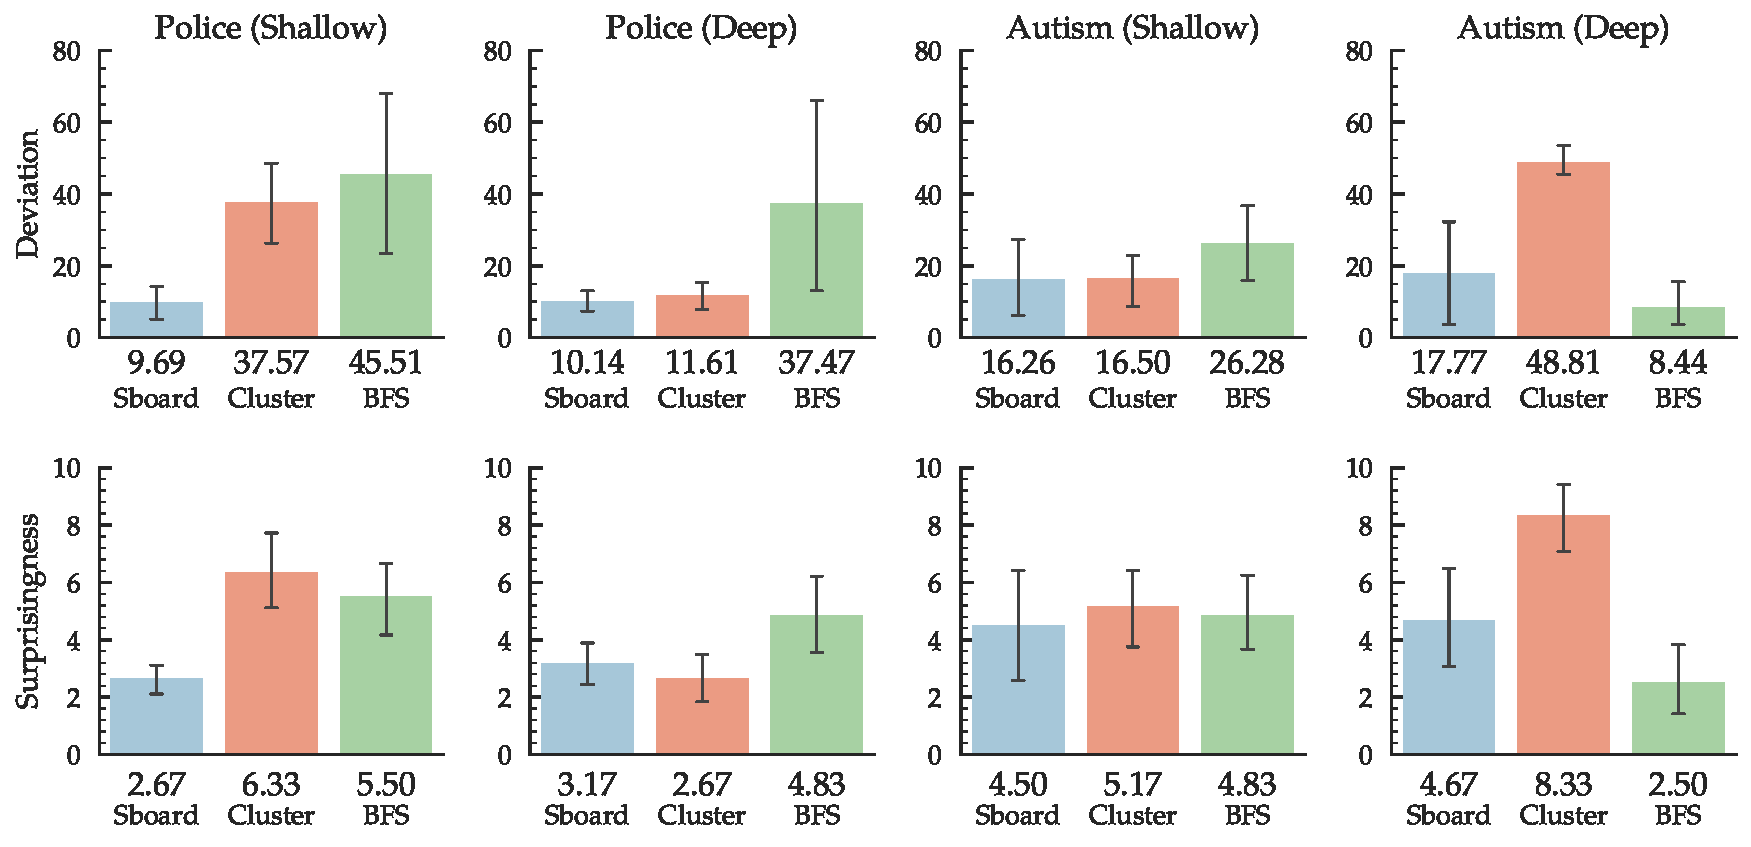
\includegraphics[width=\linewidth]{figures/Devation_Surprisingness.pdf}
\caption{Top: Euclidean distance between predicted and ground truth. Bottom: Surprisingness rating reported by users after seeing the actual visualizations on a Likert scale of 10.}
\label{fig:distance}
\end{figure*}
\begin{figure*}[bht]
\centering
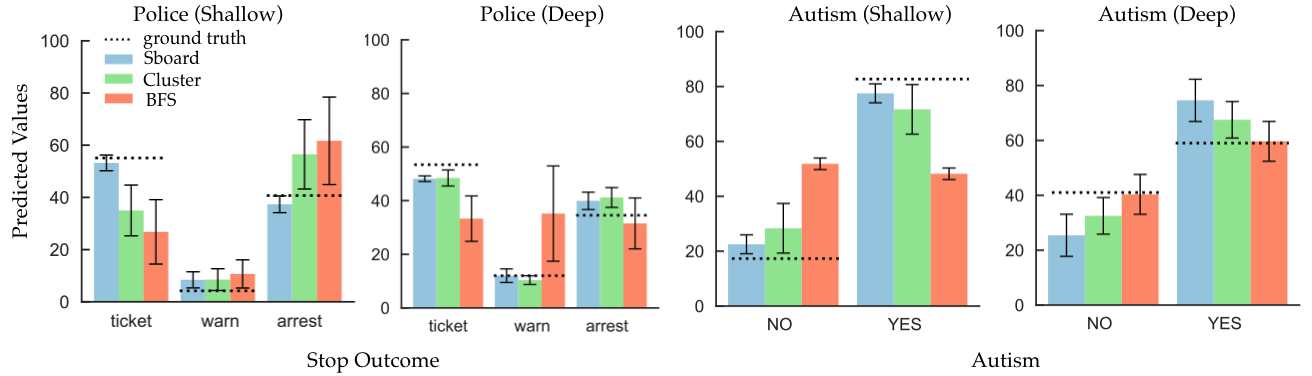
\includegraphics[width=\linewidth]{figures/Prediction_Actual.png}
\caption{Mean and variance of predicted values. Predictions based on \system exhibits lower variance (as indicated by the error bars) and great proximity to the actual values (dotted).}
\label{fig:actual_predictions}
\end{figure*}
\subsection{Qualitative results (RQ3)}
We analyzed the transcriptions of the study recordings through an open coding process by two of the authors. For each task performed by the participants, a binary-valued code is assigned to indicate whether or not the participant engaged in the particular event (action or thought process). We will refer to participants engaging in a dashboard created by algorithm=\{1,2,3\}=\{\system, \cluster, \BFS\} on dataset =\{A,B\}=\{Police, Autism\} with the notation [Participant.DatasetAlgorithm].

\stitle{\system promotes distribution-awareness by provoking comparisons against more informative contextual references.}
\par We first examined the thematic codes regarding how participants understood the context of the visualization distribution. In particular, we were interested in the types of visualizations that participants compared against in order to form their expectations regarding how other visualizations should be distributed. We define this property of visualization understanding as \textit{distribution-awareness} and the visualizations that are compared against as the \textit{contextual reference}. Via the thematic coding, we uncovered four main classes of contextual references, described below using the example visualization \texttt{gender=F, race=White, age=21-30} (in order of most to least similar):
\begin{enumerate}
	\item Parent : Comparison against a visualization with one filter criterion removed (e.g. \texttt{gender=F, race=White})
	\item Siblings : Comparison against a visualization that share the same parent. In other words, the filter types are the same, but with one criterion that inherit a different value. (e.g. \texttt{gender=M, race=White, age=21-30})
	\item Relatives : Comparison against a visualization that share some common ancestor (excluding overall), but not necessarily the same parent. In other words, these visualizations share at least one common filter type, but with more than one criterion that inherit a different value. (e.g. \texttt{gender=F, race=White, age=60+, search conducted=T})
	\item Overall : Comparison against the distribution that describes the overall population (no filters applied).
\end{enumerate}
Studying participants' use of contextual reference reveals inherent challenges in dashboard selection through \BFS and \cluster. As shown in Table \ref{table:contextualReferenceCount}, for \cluster , participants mainly compared against relatives and the overall. Since \cluster optimizes for diversity of shape distributions amongst the visualization, the selected visualization had up to 4 filters and were disconnected from each other. For this reason, in many cases participants could only rely on relatives and overall as contextual references to gain distribution-awareness. For example, [P4.A2] dislike how ``a lot of [the visualizations] are far too specific. [Pointing at visualization consisting of 4 filters with a 100\% bar for warning] This is not very helpful. You can't really hypothesize that all people are going to be warned, because it is such a specific category, it might just be one person''. %, you need to have a bigger dataset. And that category will not really give you such extremes to make it more credible''.
He further explained how he ``would not want to see the intersections (visualizations with multi-variable filters) at first and would want to see all the bases (visualization with one variable at a time) then dig in from there.'' In addition, the lack of informative contextual reference in the \cluster dashboard is reflected in the high variance and deviation of the predicted visualization results.
%despite our modification to KMeans which picks the visualizations with the least number of filters to show in the dashboard for improving interpretability
%These themes are drawn from user's explanations of how they obtained certain insights or ---- that --different tasks or while interpreting the dashboards. 4 categories :
\begin{table}[h!]
\centering
	\begin{tabular}{l|rrrr|r}
	\hline
	 Algorithm   &   Overall &   Parent &   Sibling &   Relative &   Total \\
	\hline
	 \system     &        11 &       12 &         8 &          0 &      31 \\
	 \cluster     &         8 &        4 &         0 &          7 &      19 \\
	 \BFS         &         8 &        0 &         5 &          1 &      14 \\
	\hline
	\end{tabular}
\caption{Number of participants who made use of each contextual parents, summed across the two datasets. Participant behavior shows a similar trend in individual datasets.}
\label{table:contextualReferenceCount}
\end{table}
\par For BFS, most comparisons were among overall and siblings. Due to the sequential, level-wise picking approach, in all cases for the \BFS dashboard generated, the overall corresponded to the immediate parent, so they are not explicitly recorded as parent. While the overall and sibling comparisons can be informative, due to the limited budget $k$, not all first-level visualizations were displayed in the dashboard. These incomplete comparisons can result in flawed reasoning, as observed in the Autism shallow prediction task described earlier. In contrast, for \system, users mainly compared against the overall and parents, while some also exploited sibling comparison information to make a less certain guess. We also find that more participants make comparisons in total using \system than compared to \cluster and BFS.

\stitle{Hierarchical layout leads to more natural contextual comparisons compared to table layout.}
\par As described in the previous section, contextual parents are important in establishing distribution-awareness for understanding the dataset. Participants cited hierarchical layout as one of the key reasons why it was easier to follow contextual reference in \system. Based on the hierarchical layout in \system, users were able to easily interpret the meaning of the dashboard, even though they were never explicitly told what the edge connections between the visualizations meant. For example, [P1.A1] stated that ``the hierarchical nature [is] a very natural flow...so when you are comparing, you don't have to be making those comparisons in your head, visually that is very pleasing and easy to follow.'' %Likewise, [P8.A1] also stated that ``I like the different levels, it makes it very visually easy to figure out what you want to look at, if you want to look at the overall data, it's right there at the top for you, if you want to get more specific, you just follow a branch downwards, which I think is very intuitive.''
Likewise, P9 described how the hierarchical layout she saw for the Autism dataset was a lot easier to follow than the Police dataset shown in the table layout:
\begin{quote}
If I had to look at this dataset in the format of the other one, this would be much more difficult. It was pretty hard for me to tell in the other one how to organize the tree, if there was even a tree to be organized. I like this layout much better, I think this layout allows me to approach it in a more meaningful way. I can decide, what do I think matters more: the overall trend? or the super detailed trends? and I know where to look to start, in the other one, every time I go back to it, I would say, where's the top level, where's the second level? I mentally did this. Like when you asked me that first question, it took much longer to find it, because I literally have to put every chart in a space in my head and that took a lot longer than knowing how to look at it.
\end{quote}
At the end of the study, some participants for \BFS and \cluster sketched and explained how they would like the layout of the visualizations to be done. Participants expressed that they wanted ``groupings'' or layouts that arranged visualizations with the same attribute together. Other participants advocate for isolating the overall visualization outside of the dashboard table for facilitating easier comparisons. Both of these provides further motivation for our hierarchical layout and the idea of the collapsed visualizations as described in Section \ref{sec:interaction}.
\par Since we did not inform participants how the dashboards were generated, it was also interesting to note that some participants thought that the dashboards were hand-picked by a human analyst and described what this person's intentions were (e.g. ``It seems like the researcher who created this dashboard was specifically looking at people of Asian descent and people who are 60 or older.'' [P7.A1]). We encoded this phenomenon by looking at instances where a participant either explicitly referring to a person who picked out the dashboard or implicitly described their intentions through personal pronouns. A total of 5 different participants referred to the dashboard generated by \system as generated by a human, whereas there was only 1 participant for \cluster and none for \BFS made such remarks. At the end of the study, many were surprised to learn that the \system dashboard was actually picked out by an algorithm, indicating that \system could automatically generate convincing dashboard stories that were similar to a dashboard that was authored with intention.

\stitle{Improper contextual reference can lead to misleading insights.}
\par While comparisons are essential for data understanding, choosing the wrong contextual reference for comparison could lead to misleading insights. In particular, when a visualization that is composed of multiple filter conditions is shown in a dashboard created using \cluster, 5 out of 12 participants for both datasets had a hard time interpreting the meaning of the filter, whereas there was only 1 for \system and BFS. This is due to the fact that \cluster dashboards are seemingly random to the users, whereas \BFS and \system both have some natural ordering. In addition, when examining visualizations with many filters and contain bars that exhibit extreme values (bars with 100\% or 0\% in one or more categories), 4 \cluster participants did not realize that charts with multiple filters may have a smaller subpopulation size. This issue stems from the fact that the contextual reference used for comparison was the overall population, however the unseen parent subpopulation may have behaved very differently. The fallacy was observed to be more severe for the Autism dataset, where participants had less intuition on the expected attribute behavior. In contrast, 6 of the participants using \system recognized that while these extreme-valued visualizations may be interesting, they were less certain due to the unknown subpopulation size and should be investigated further. For example, [P1.A1] noted that a visualization with warning=100\% caught her eye, ``but I don't know what the N is, maybe it's one person, this makes me a little skeptical, that makes me want to go back to the raw data and look at what is the N and what drives something so drastic?''. Since \BFS dashboards only displayed first-level visualizations, participants for \BFS did not see such visualizations during the study session, so we did not see signs of this fallacy for \BFS participants.

\stitle{Limitations of \system}
\par As described earlier, since the details of how the dashboard was obtained was not explained to the users during the study, some users expressed that they were initially confused by \system since not all variables were present in the dashboard and others found it confusing that the addition of filters did not always correspond to the same variables. For example, [P2.A1] criticized how the dashboard was intentionally selected to be biased:
\begin{quote}
I feel like this one, not all the data is here, so we are already telling a story, you are trying to steer the viewer to look at certain things. And the focus seems to be on where the arrest rate is high. You probably could have found other things that led to ticket being high, but you didn't pull those out. You are trying to see if there are other factors that leads to more arrests.
\end{quote}
\npar This sentiment is related to participants' desire to perform their own ad-hoc querying alongside the dashboard to inspect other related visualizations for verifying their hypothesis. For example, [P7.A1] wanted to inspect all other first-level visualizations for driver's race to assess its influence. [P7.A1] expressed that while he had learned many insights from the dashboard, ``the only thing I don't like is I can not control the types of filter, which is fixed.'' Outside the context of the user study, it is essential to explain how \system are picking the visualizations in a easy and interpretable manner to establish a sense of summarization guarantee for the users and help them make better inferences with the dashboard.
\par As discussed earlier, subpopulation size is important in establishing the `credibility' of a visualization. While subpopulation size is taken into account implicitly in our objective (as described in Section~\ref{sec:utility}), we should design interfaces that can convey the notion of subpopulation size in our dashboard, either explicitly displayed as text when hovering over the visualization or changing the size or background color of the visualizations to encode subpopulation size.
%“I actually found it really confused at first because such a low arrest rate at the top, and then at the bottom the arrest rate was much higher, so I was like is this data wrong. Then I realized we’re not looking at all the data here, you’ve pulled out some of it. It took me a minute to realize that. And once I read the title of the charts I realized that makes sense.” [P2.A1]
% - Reference of Comparison
% - Layout naturally lends itself for comparison:
% 	- describe ordering layout, how participants naturally follow the flow
% 	- emph that we did not tell them what the edge connections mean and how they were computed but the users naturally figured it out, that it means adding an additional filter.
% 	- hierarchical interpretable nature (quotes)
% 	- compared to other baselines
% 	- describe dashboard by human (count)
% - Misleading insights v.s. True insight discovery rates
% 	- Interpretability:
% 	- misled understanding subpopulation size
% 		- for autism, it is important to see if they compare to overall because if not they would think high skew to NO is important whereas its actually pretty close to overall.
% 	- trouble interpreting filter combination

%!TEX root = main.tex
\section{Discussion}
\subsection{Statistical Paradoxes}\dor{make title full sentences}
Visualizations are powerful representations for studying different distributions or patterns in a dataset, but our human intuition could often misleads us when it comes to interpreting those patterns\cite{Binnig2017,Wall2017}. Several statistical paradoxes can lead analysts to draw incorrect conclusions from observed visualizations, including Simpson's paradox as discussed in the introduction. The key reason why many of these paradoxes emerge is the \emph{incompleteness} of the observed data or lack of focus on relevant informative subsets of the data. For example, Simpson's paradox arises in the presence of an unseen confounding variable. %likewise, the absence of  base rate information causes base rate fallacy.
 We assert \dor{too strong of a sentence} that distributional awareness can be useful in avoiding such statistical paradoxes. If an analyst is aware of all distributions in a given dataset, he/she is less prone to many statistical paradoxes. However, given the large number of dimensions and high cardinality of these dimension in modern datasets, it is not possible for an analyst to explore and memorize all distributions. Therefore, a more evolved approach is to be aware of the exceptional distributions. In this work, we propose a first step towards this goal, where we identify the exceptional distributions in terms of their informative references. The remaining (unseen) distributions in the dataset are rather unsurprising and can be inferred from the visualizations in the dashboard. \dor{I would recommend first talk about issue with large dimension + danger of multiple hypothesis testing + incomplete testing, point out problem, then talk about how our system resolves this.}

\subsection{Structural Insight}
Our proposed dashboard consists of a hierarchy of visualizations, where each visualization is linked to its most informative parent. The shape or structure of the hierarchy contains useful information that augments the information learned from the visualizations and aid distribution awareness and understanding. \dor{what's interesting here is that while many work have looked at visualization presentation, layout of presentation never considered, we find in Sec 5 that this is actually important and can encode info.} For example, the depth and branching factor of the hierarchy could inform a user regarding the configuration of insights. Deep hierarchies contain long paths, i.e., insights are present at lower level visualizations with multiple constraints. In contrast, bushy hierarchies (with high branching factor) contain cases where multiple visualizations have the same informative parent and they differ from that parent. \dor{do we have examples from the study that support this?} We assert that the depth and branching factor could be a meaningful constraint in our problem formulation \dor{too strong of a sentence}. Some applications for example, funnel exploration require studying deep hierarchies, whereas others for example, building decision trees require studying bushy hierarchies. A natural extension of our current problem formulation is to allow users to select the depth and branching factor for the hierarchy. 

\subsection{Other Visualization Lattices}
In this work, we explore the space of data subsets to generate our visualization lattice. Note that it is possible to explore the space of dimension attributes in x-axis to generate a different visualization lattice. In particular, given a combination of dimension attributes $X = \{X_1, \ldots, X_n\}$, adding one or more new dimensions in $X$ will generate a new combination. An ancestor-descendant relationship exists between these dimension combinations, following the same principles of Section 3.1. These relationships lead to a new lattice, which we call the dimension combination lattice. Our informative deviation based approach could be used for traversing the dimension combination lattice. However, we observe that most users do not visualize more than two attributes in x-axis. Therefore, traversing the dimension combination lattice is not very useful for most applications.
\dor{I think 6.2,6.3 don't tie well with the rest of the paper. It sounds like stretching our own ideas rather than being motivated by the work done in this paper. Other potentially more relevant discussion: distribution awareness and how it might be useful in other contexts? Decision trees?}
%\subsection{Utility Metrics} 




%!TEX root = main.tex
\section{Related Works}
\npar \stitle{Storytelling with visualization sequences:}
Visualizations are often arranged in sequence to narrate a data story. Existing work on visualization sequences and storytelling have studied the structures of narrative visualizations\cite{Segel2010,Hullman2017}, effects of augmenting exploratory information visualizations with narration\cite{Boy2015} and, more recently, ways to automate the creation of visualization sequences\cite{Hullman2013,Kim2017}. Most of these work have adopted a linear layout (motivated by slidedecks) to present the visualization sequences. Hullman et al. \cite{Hullman2017} found that most people prefer visualization sequences structured hierarchically based on shared data properties such as levels of aggregation. %Both \cite{Hullman2013,Kim2017} use a graph model to formalize the visualization design space.
Kim et al. \cite{Kim2017} models relationships between charts by empirically estimating transition (edge) cost between moving from one visualization (node) to another. They find that participants preferred ``\textit{starting from the entire data and introducing increasing levels of summarization}''. Our work is the first to automatically sequences visualizations in a hierarchical layout for summarizing the space of data subsets. %In addition, we present a novel problem formulation that recommends a connected visualization sequence in a hierarchical layout summarizing the space of data subsets.

\subsection{Visualization recommendation}
\par%Despite the large body of work that recommends informative visualizations given pre-selected data attributes and aggregations, the data selection problem is a more important problem in exploratory data analysis, since the analysts have to figure out which groups of data attributes would be of interest in order avoid manual exploration of the data.
Visualization recommendation systems select appropriate visualizations to show based on an objective function. The metrics considered by these systems can largely be divided into two categories: perceptual or data-driven. The first type of recommendation system selects visualizations based on its visual effectiveness and expressiveness~\cite{Wongsuphasawat2016,Mackinlay2007}. Our work is more related to the latter category of systems which uses statistical measures computed based on the underlying data subset, such as cognostics or deviation. Anand et al. \cite{Anand2015} used randomized permutation tests to automatically select partitioning variables upon to display visualizations exhibiting patterns that are different from the input visualization as determined by its cognostic score. Vartak et al. \cite{Vartak2015} finds interesting visualizations by a deviation-based measure between the user's query view and reference view, given a query of interest. While both existing systems require the analyst to input a visualization of interest as a query, our paper extends the deviation-based idea to establish user's expectation using informative parent enabling \system traverse the visualization lattice in search of a connected, maximally informative and interesting story without the need for an input query.  %Wongsuphasawat et al. \cite{Wongsuphasawat2016} presents a mixed-initiative system where the users direct the variables of interest and the system suggests other variables that may be potentially interesting to the user. Since this is a mixed-initiative system rather than an automatic recommendation engine, the system only ``looks ahead" one variable at a time. Their goal is to promote breadth-oriented data exploration rather than helping users find interesting stories or visualizations.

%- the issue of surprisingness metric and ---- have been examined before for viz, but none have looked at data subset lattice specifically for viz

\subsection{Data Exploration of OLAP Data Cubes} %\dor{This may be a bit long and need to be cut, I didn't include related works on surprisingness metrics (e.g. Bayesian Cognition paper, Surprise Map ,etc.). Can add if necessary.}
The challenge of manual, unguided search in online analytical processing (OLAP) applications have been well studied in the context of data cube exploration by Sarawagi et al. ~\cite{Sarawagi1999,Sarawagi2000,Sarawagi1998}. To address this challenge, they simplify the search by identifying ``interesting'' regions of a data cube. These techniques includes precomputed statistics accounting for the surprisingness attributed to neighboring paths to cell and amount of deviation from constrained maximum entropy-based expectations. While these interesting sub-cubes correspond to finding filter combinations for constructing the aggregate visualization in \system, our lattice search space enforces fixed x, y and aggregation as well as connectedness during traversal to discover more interpretable stories.

%Sarawagi et al.\cite{Sarawagi1998} introduced the problem that manual, unguided search for seeking interesting patterns in a datacube is inefficient and requires large numbers of online analytical processing (OLAP) operations, such as roll-up, drill-down, slicing, and dicing. They proposed a discovery-driven approach to data exploration to simplify the search for \textit{exceptions} in the data, based on precomputed statistics regarding how surprising a data cube cell is, relative to neighboring cells at the same level of aggregation, at levels of aggregation below the cell, and along the drill-down path. Sarawagi \cite{Sarawagi1999} presents an OLAP operator that summarizes the reasons for variation in a data view, by computing the information theoretic distance between the immediate parent and its child nodes.
% \par While Sarawagi et al. \cite{Sarawagi1998} takes a more data-driven approach of finding exceptions intrinsic to a given datacube, Sarawagi \cite{Sarawagi2000} envisions a more user-centric application where the comparisons are based only on parents of seen visualization. The user's expectation regarding an unseen visualization is based on the maximum entropy principle where the relationships between the attributes should be maximally uniform across all dimensions, while being consistent with constraints from seen visualizations. The visualization that deviates the most from the user expectation is regarded as an ``interesting" visualization. They take an iterative approach to find the unique solution for the expected values for each attribute from the constrained maximum entropy problem and employ several optimization strategies (reusing computed values, sharing storage of contiguous regions, pruning constraints that subsumes one another or with little influence). Our coverage-based models improve on the iterative approach in providing a tighter constraint to the variable regions of the bars.

%!TEX root = main.tex
\section{Conclusion}


% \bibliographystyle{abbrv}
\bibliographystyle{abbrv-doi}
\bibliography{reference}

\end{document}
